% ============================================================
% main.tex — Plantilla genérica para usar con uti_tfm.sty
% Requiere en la misma carpeta del proyecto:
%   - uti_tfm.sty
%   - referencias.bib
%   - Logos/LOGO-UTI.png
%
% Compilación recomendada (por Century Gothic):
%   XeLaTeX → biber → XeLaTeX → XeLaTeX
% ============================================================

\documentclass[12pt,a4paper,oneside]{report}

% Estilo UTI
\usepackage{uti_tfm}

% Referencias IEEE desde .bib (usa biber)
\usepackage[hidelinks]{hyperref} % opcional pero recomendado
\renewcommand{\bibname}{REFERENCIAS} % report/book
% (si fuera article sería \renewcommand{\refname}{REFERENCIAS})


\usepackage{tikz}
\usetikzlibrary{positioning,shapes.geometric,arrows.meta,calc}
% Útiles (opcionales)
\usepackage[hidelinks]{hyperref}
\usepackage{graphicx}
\usepackage{longtable}
\usepackage{csquotes}


\begin{document}

% ==========================================================
% PORTADA (sin numeración visible; NO cuenta para la numeración)
% ==========================================================
% Géneros permitidos: masculino | femenino
% Cada autor/a debe llenar sus propios datos con el comando correspondiente:
%   \UTIDatosAutorUno{Nombre completo}{género}{cédula}{dirección}{correo}{teléfono}
%   \UTIDatosAutorDos{Nombre completo}{género}{cédula}{dirección}{correo}{teléfono}
% Si solo hay un/a autor/a, omite \UTIDatosAutorDos.
\UTIPortada
{LOGO-UTI-1.png} % Logo (ruta)
{FACULTAD DE INGENIERÍAS} % Facultad
{INGENIERÍA EN TECNOLOGÍAS DE LA INFORMACIÓN} % Programa
{Diseño de un gemelo digital de una empaquetadora de arroz} % Tema / Título
{Trabajo de Titulación modalidad Trabajo de Integración Curricular} % Texto tipo de trabajo
{%
  \UTIDatosAutorUno{Kiany Scarleth Cárdenas Burbano}{femenino}{1727133603}{Provincia, ciudad, parroquia, barrio}{kiany.correo@ejemplo.com}{0999999999}%
  \UTIDatosAutorDos{Bryan David Toaza Yandún}{masculino}{1756142392}{Provincia, ciudad, parroquia, barrio}{bryan.correo@ejemplo.com}{0999999999}%
} % Autor/a(s)
{\UTIDatosTutor{Andrés Xavier Rubio Proaño}{masculino}} % Tutor/a
{Quito, Ecuador} % Ciudad, País
{2026} % Año

% ==========================================================
% PÁGINAS PRELIMINARES (romanos minúscula: i, ii, iii...)
% ==========================================================
\UTIFrontMatter

\input{Preliminares/01_RepositorioDigital}

\input{Preliminares/02_AprobaciónTutor}

\input{Preliminares/03_DeclaraciónAutenticidad}

\input{Preliminares/04_AprobaciónLectores}


\UTIIfTwoAuthorsTF{%
\UTIFrontTitle{Dedicatoria}

\vfill

\begin{flushright}
\textbf{\UTIAutorUnoNombre}\\
Este trabajo deja recuerdos de largas jornadas de trabajo en la mejor compañía; este logro es dedicado con cariño a Bryan Toaza porque también le pertenece, sin su ayuda no lo habría alcanzado.
\end{flushright}

\UTIFrontTitle{Dedicatoria}

\vfill

\begin{flushright}
\textbf{\UTIAutorDosNombre}\\
(Obligatoria)\\
La dedicatoria de este autor o autora va en la parte inferior derecha de la página.
\end{flushright}
}{%
\UTIFrontTitle{Dedicatoria}

\vfill

\begin{flushright}
(Obligatoria)\\
La dedicatoria va en la parte inferior derecha de la página.
\end{flushright}
}

\UTIIfTwoAuthorsTF{%
\UTIFrontTitle{Agradecimiento}

\vfill

\begin{flushright}
\textbf{\UTIAutorUnoNombre}\\
Culmino esta etapa agradecida con Dios, con su bendición pude recorrer este camino junto a mi madre, Blanca, y mi abuela, Carmen, cómplices de este logro; por su trabajo incansable, amor y apoyo, mi eterno reconocimiento. Y a mis maestros por compartir conocimiento y amistad.
\end{flushright}

\UTIFrontTitle{Agradecimiento}

\vfill

\begin{flushright}
\textbf{\UTIAutorDosNombre}\\
(Obligatorio)\\
El agradecimiento de este autor o autora va en la parte inferior derecha de la página.
\end{flushright}
}{%
\UTIFrontTitle{Agradecimiento}

\vfill

\begin{flushright}
(Obligatorio)\\
El agradecimiento va en la parte inferior derecha de la página.
\end{flushright}
}



% --------------------------
% ÍNDICES (según el .sty)
% --------------------------
\input{Preliminares/07_Índices}

\input{Preliminares/08_Resumen}

\input{Preliminares/09_Abstract}
% ==========================================================
% CUERPO (arábigos CONTINUANDO el contador desde los romanos)
% Nota: el .sty cambia el formato de página a arábigos sin reiniciar.
% ==========================================================
\UTIMainMatter

% ==========================================================
% CAPÍTULO I (se mostrará como: CAPÍTULO I)
% ==========================================================
\chapter{Introducción}
\label{chap:introduccion}

% ==========================================
\section{Contextualización}
% ==========================================

La globalización de las cadenas de suministro agroindustriales ha generado una presión sin precedentes sobre los sistemas de manufactura y procesamiento de alimentos. En la última década, la Industria 4.0 ha emergido como un paradigma transformador que fusiona activos físicos con tecnologías digitales para crear sistemas ciberfísicos \cite{monostori2016}. En este contexto, la República del Ecuador presenta un escenario dual: mientras el sector agroindustrial representa un pilar fundamental de su Producto Interno Bruto (PIB), la tasa de adopción de tecnologías habilitadoras de la Cuarta Revolución Industrial en las Pequeñas y Medianas Empresas (PYMES) y centros de investigación de la región latinoamericana aún se encuentra en una fase de maduración temprana.

Según las cifras reportadas por las estadísticas oficiales de producción, la transformación de granos como el arroz y el maíz constituye uno de los mayores volúmenes de procesamiento industrial en el país. Sin embargo, múltiples estudios en ingeniería de procesos han demostrado que los métodos de dosificación electromecánica tradicional presentan mermas operativas que oscilan entre el 3\% y el 5\% debido a ineficiencias en la calibración y el control reactivo de la maquinaria. Estas pérdidas, generalmente por derrames o empaques deficientes, reflejan una necesidad urgente de modernización tecnológica que no siempre puede ser satisfecha mediante la adquisición de nuevos equipos, sino a través de la transformación digital de los activos existentes.

El presente proyecto de investigación se origina en el Laboratorio de Procesos de la Universidad Indoamérica, un espacio dedicado a la validación técnica y la docencia especializada. Dentro de este laboratorio opera una máquina dosificadora de granos considerada un activo de alto valor educativo. Conceptualmente, esta máquina es una representante típica de la maquinaria \textit{legacy} industrial: opera mediante un circuito de potencia a 220V, controlado por un Controlador Lógico Programable de arquitectura cerrada, el cual gobierna una secuencia de relés y electroválvulas neumáticas para ejecutar el ciclo de dosificación. A pesar de su robustez mecánica, la arquitectura cerrada impuesta por el fabricante y las políticas de mantenimiento institucionales impidieron cualquier manipulación o perforación del tablero eléctrico original, condenando a este valioso recurso a funcionar como una ``caja negra''.

Ante esta limitación física, la solución propuesta trasciende el simple monitoreo para adentrarse en el ámbito de los Gemelos Digitales predictivos. Se diseñó una integración ciberfísica no invasiva, mediante un sistema de ``bypass'' externo gobernado por microcontroladores ESP32, que permite capturar las señales críticas del proceso sin alterar el cableado interno del PLC. A través de esta arquitectura, se replica digitalmente el comportamiento completo de la máquina, habilitando un entorno de simulación y validación que respeta la integridad del sistema original, un enfoque que marca la diferencia entre una simple réplica visual y un Gemelo Digital funcional de Nivel 3.

% ==========================================
\section{Estado del Arte}
% ==========================================

\subsection*{Evolución de los Gemelos Digitales y los CPS}
En la esfera de la manufactura inteligente, el concepto de Gemelo Digital ha evolucionado desde la mera gestión del ciclo de vida del producto hasta convertirse en un habilitador crítico para la simulación predictiva. Tao \textit{et al.} \cite{tao2019} establecieron una taxonomía de madurez que clasifica los gemelos en varios niveles, desde el monitoreo (Nivel 1) hasta la autonomía prescriptiva (Nivel 4). Para esta investigación, el foco se sitúa en el Nivel 3 (Predictivo/Interactivo), donde el modelo virtual no solo recibe datos en tiempo real, sino que puede interactuar con el sistema físico para anticipar fallos. Paralelamente, la arquitectura de referencia de 5 Niveles para CPS propuesta por Lee \textit{et al.} \cite{lee2015} provee el marco estructural para la implementación del bypass ciberfísico, permitiendo una transición fluida entre la adquisición de datos locales y el procesamiento analítico en el ciberespacio.

\subsection*{Tecnologías de Control y Simulación}
La naturaleza secuencial de las máquinas dosificadoras convierte a la teoría de control de eventos discretos en un área de estudio fundamental. Cassandras y Lafortune \cite{cassandras2021} formalizaron el uso de las Máquinas de Estados Finitos como un modelo determinístico ideal para sistemas industriales que transitan entre estados excluyentes (neumático extendido, retraído, sellado, etc.). Su implementación en Python dentro de entornos de simulación 3D como Webots \cite{michel2004} representa un avance significativo frente a los simuladores puramente matemáticos, ya que permite modelar fenómenos físicos complejos como colisiones, cinemática y gravedad. Rasheed \textit{et al.} \cite{rasheed2020} destacan que la principal barrera en el modelado predictivo suele ser la pobreza de datos, un desafío inherente a las máquinas legacy que no cuentan con sensórica inteligente nativa.

\subsection*{Protocolos de Comunicación IIoT y SCADA}
El Internet Industrial de las Cosas ofrece la columna vertebral comunicacional para estos sistemas. El protocolo MQTT, analizado en profundidad por Hunkeler \textit{et al.} \cite{hunkeler2008} y materializado en broqueros como Mosquitto \cite{light2017}, se destaca por su modelo de publicación/suscripción ligero, ideal para la telemetría bidireccional entre el ESP32 y el panel de control. A nivel de supervisión, Node-RED, fundamentado en la investigación sobre flujos de datos distribuidos de Blackstock y Lea \cite{blackstock2014}, ha desplazado en entornos académicos a los SCADA propietarios tradicionales debido a su flexibilidad y capacidad de integración visual. Autiosalo \textit{et al.} \cite{autiosalo2020} complementan este enfoque proponiendo una arquitectura basada en características para estructurar los gemelos digitales, facilitando la rastreabilidad de los datos y la interoperabilidad de los componentes.

\subsection*{Casos de Estudio en Maquinaria Legacy}
Aunque la literatura documenta ampliamente aplicaciones de gemelos digitales en máquinas herramienta CNC y robots de última generación \cite{qi2018}, existe una notable escasez de aplicaciones prácticas en equipos de manufactura brownfield/legacy. La investigación de Monostori \textit{et al.} \cite{monostori2016} sobre CPS en manufactura identifica precisamente esta brecha, señalando la dificultad de extraer datos significativos de infraestructuras antiguas sin tiempos de inactividad extensos o inversiones prohibitivas. Es en esta intersección donde la presente tesis realiza su principal contribución científica.

A continuación, en la Tabla \ref{tab:estado_arte}, se presenta una clasificación detallada de los principales hallazgos bibliográficos que constituyen el soporte científico del proyecto.

% --- INICIO DE LA TABLA CONFIGURADA PARA DIVIDIRSE EN VARIAS PÁGINAS ---
{\footnotesize
\renewcommand{\arraystretch}{1.3}
\begin{longtable}{|c|p{1.5cm}|p{3.2cm}|p{2.5cm}|p{2cm}|p{3cm}|}
\caption{Clasificación de la literatura revisada para el estado del arte.}
\label{tab:estado_arte} \\
\hline
\textbf{N°} & \textbf{Autor(es) y año} & \textbf{Título abreviado} & \textbf{Tecnología principal} & \textbf{Aplicación} & \textbf{Limitación identificada} \\
\hline
\endfirsthead

% Encabezado para las páginas siguientes
\multicolumn{6}{c}%
{{\tablename\ \thetable{} -- Continuación de la página anterior}} \\
\hline
\textbf{N°} & \textbf{Autor(es) y año} & \textbf{Título abreviado} & \textbf{Tecnología principal} & \textbf{Aplicación} & \textbf{Limitación identificada} \\
\hline
\endhead

% Pie de tabla final (al terminar todos los datos)
\hline
\endlastfoot

1 & Tao et al. (2019) & ``Digital Twin in Industry'' \cite{tao2019} & Gemelo Digital (Niveles 1-4) & Manufactura general & Marco conceptual sin validación en bypass ciberfísico. \\ 
\hline
2 & Lee et al. (2015) & ``A CPS Architecture for Industry 4.0'' \cite{lee2015} & CPS 5 Niveles & Sistemas de manufactura & Arquitectura de alto nivel, sin implementación práctica en dosificadoras. \\
\hline
3 & Monostori et al. (2016) & ``CPS in Manufacturing'' \cite{monostori2016} & CPS & Manufactura general & Enfoque macro, no aborda modernización de equipos brownfield. \\
\hline
4 & Rasheed et al. (2020) & ``Digital Twin: Values, Challenges and Enablers'' \cite{rasheed2020} & Modelado de Gemelo Digital & Gestión de activos & Requiere alta fidelidad de datos, ausentes en máquinas sin sensórica nativa. \\
\hline
5 & Michel (2004) & ``Webots: Professional Robot Simulation'' \cite{michel2004} & Simulación 3D (Webots) & Robótica móvil & Orientado a robótica, no a maquinaria industrial fija de eventos discretos. \\
\hline
6 & Cassandras \& Lafortune (2021) & ``Introduction to Discrete Event Systems'' \cite{cassandras2021} & Máquina de Estados Finitos (FSM) & Control Secuencial & Alta complejidad formal para traducción directa a microcontroladores. \\
\hline
7 & Hunkeler et al. (2008) & ``MQTT-S Protocol'' \cite{hunkeler2008} & Protocolo MQTT (IoT) & Redes de sensores & Enfoque en sensores simples, no en acoplamiento con gemelos 3D en tiempo real. \\
\hline
8 & Blackstock \& Lea (2014) & ``Distributed Data Flow for WoT'' \cite{blackstock2014} & Node-RED / SCADA & Web of Things (WoT) & Escasez de integración directa con simuladores físicos educativos o dashboards FSM. \\
\hline
9 & Qi \& Tao (2018) & ``Digital Twin and Big Data'' \cite{qi2018} & Gemelo Digital \& Big Data & Manufactura Inteligente & Dependencia de grandes volúmenes de datos, ausentes en máquinas legacy. \\
\hline
10 & Autiosalo et al. (2020) & ``Feature-Based Digital Twins'' \cite{autiosalo2020} & Estructura de DT & Manufactura & No aborda despliegue en sistemas con restricciones físicas de manipulación. \\
\end{longtable}
}
% --- FIN DE LA TABLA ---

\subsection{Brecha de Investigación}
A partir de la revisión sistemática presentada, se identifica una brecha de investigación significativa en la integración de Gemelos Digitales de Nivel 3 para maquinaria electromecánica heredada que carece de puertos de comunicación modernos. La literatura actual está dominada por trabajos que asumen conectividad nativa o capacidad de modificación total del hardware, una condición que rara vez se cumple en los laboratorios universitarios y las PYMES agroindustriales ecuatorianas. Esta tesis aborda dicha carencia mediante el diseño de un bypass ciberfísico basado en ESP32 y MQTT, validando un modelo no invasivo que emula fielmente la cinemática y la lógica de control secuencial de una dosificadora industrial, sin violar la integridad del controlador original.

% ==========================================
\section{Planteamiento del Problema}
% ==========================================

La máquina dosificadora de granos ubicada en el Laboratorio de Procesos de la Universidad Indoamérica representa un quebranto tecnológico para el desarrollo académico de la institución. A pesar de ser completamente funcional, su arquitectura de control presenta serias limitaciones para la investigación en Industria 4.0. El sistema opera bajo una filosofía de control de lazo cerrado y opaco: un PLC propietario enclavado a un contactor trifásico de 220V ejecuta la lógica de electroválvulas y pistones en un ciclo estrictamente secuencial. Esta configuración impedía cualquier forma de extracción de datos en tiempo real o modificación paramétrica externa.

La situación problemática actual se define por tres causas raíz interrelacionadas. En primer lugar, la política de no manipulación interna del equipo (impuesta para preservar la integridad del equipo de docencia) bloqueaba la instalación de sensores de corriente en el gabinete de control. En segundo lugar, la naturaleza \textit{legacy} del equipo implica la ausencia total de buses de comunicación industrial modernos (Modbus/TCP, Profinet, EtherCAT) que permitan una telemetría directa. Finalmente, las restricciones presupuestarias del laboratorio de investigación descartaban la opción de reemplazar la unidad por un equipo de última generación.

Los efectos de esta situación se traducen en tiempos de inactividad no programas por la falta de mantenimiento predictivo, la pérdida continua de trazabilidad en los lotes de dosificación procesados, y la imposibilidad técnica de desarrollar prácticas de posgrado orientadas a la transformación digital. Como consecuencia, el laboratorio opera actualmente bajo un esquema de mantenimiento exclusivamente reactivo, desaprovechando los recursos de instrumentación y control modernos.

A la vista de esta problemática, surge la siguiente pregunta de investigación: \textbf{¿Cómo diseñar e implementar un gemelo digital predictivo e interactivo para una máquina dosificadora de granos, sin necesidad de modificar su estructura interna de control, mediante el uso de un bypass ciberfísico que garantice la interoperabilidad con tecnologías IIoT?}

% ==========================================
\section{Justificación}
% ==========================================

El desarrollo se justifica desde cuatro perspectivas estratégicas que consolidan su pertinencia técnica y académica.

En el ámbito \textbf{técnico}, la solución propuesta introduce el concepto de ``bypass ciberfísico'' como una alternativa no invasiva para la modernización industrial. A diferencia de los métodos convencionales que requieren el reemplazo total del sistema de control, el diseño implementado conecta una capa de inteligencia externa (ESP32, MQTT, Node-RED) sin perforar ni modificar el cableado original del PLC. Esto constituye una contribución metodológica para la interoperabilidad de sistemas brownfield en el paradigma de la Industria 4.0, validando la sinergia entre tecnologías de hardware abierto y software libre como Webots, Python y FreeCAD.

Desde el punto de vista \textbf{operativo}, la migración de la dosificadora hacia un gemelo digital predictivo busca minimizar las mermas y las interrupciones del servicio. Al habilitar la monitorización en tiempo real a través del broker MQTT Mosquitto y el panel SCADA en Node-RED, se elimina la dependencia del mantenimiento netamente reactivo. La generación de métricas de rendimiento, latencias y detección de fallos provee a los investigadores y docentes de una herramienta cuantitativa para optimizar la dosificación de granos, un hecho que incide directamente en la reducción de pérdidas por mermas estimadas entre el 3\% y 5\%.

La justificación \textbf{académica} radica en la capacidad de transferencia del conocimiento generado. Al ser un proyecto de código abierto, constituye un caso de estudio replicable en otros laboratorios universitarios de Iberoamérica que enfrentan el desafío de actualizar equipamiento industrial obsoleto sin grandes inversiones.

Finalmente, la viabilidad \textbf{económica} es un factor crítico. La implementación se sustenta enteramente en tecnologías de bajo costo y amplia disponibilidad en el mercado local. Frente al costo de una dosificadora industrial moderna con conectividad IIoT nativa, el prototipo diseñado representa un costo marginal, ofreciendo un retorno de inversión inmediato al convertir un activo subutilizado en una plataforma de validación tecnológica de alto nivel.

% ==========================================
\section{Objetivos}
% ==========================================

\subsection{Objetivo General}
Desarrollar un gemelo digital interactivo y predictivo de una máquina dosificadora de granos mediante la integración del motor de simulación Webots, una arquitectura de Máquina de Estados Finitos (FSM) y un bypass ciberfísico basado en ESP32, para emular fielmente la cinemática del ciclo industrial y habilitar la validación algorítmica de métricas de rendimiento y resiliencia ante escenarios de falla en un entorno ciberfísico seguro.

\subsection{Objetivos Específicos}
\begin{enumerate}
  \item \textbf{Levantar y diagnosticar} la lógica secuencial y los parámetros operativos de la dosificadora electromecánica y su controlador base, definiendo la topología de la red de información, los tiempos de latencia del sistema físico y los puntos críticos de instrumentación para la integración ciberfísica.
  \item \textbf{Diseñar e implementar} el modelo ciberfísico en Webots, programando una FSM en Python que gobierne de manera aislada la cinemática de los actuadores (alimentación, dosificación y sellado), integrando la telemetría mediante el protocolo MQTT y el panel SCADA en Node-RED, y ejecutando el bypass que respete la integridad del sistema original.
  \item \textbf{Evaluar} la resiliencia y eficiencia de la lógica de control mediante la inyección de perturbaciones virtuales (fallos de presión y lectura), cuantificando el impacto en el rendimiento operativo, la capacidad de detección de anomalías y la efectividad general del sistema frente a escenarios de falla simulados.
\end{enumerate}

% ==========================================
\section{Alcance del Proyecto}
% ==========================================

El proyecto se circunscribe al diseño, desarrollo y validación de un Sistema Ciberfísico de Nivel 3 (Gemelo Predictivo e Interactivo), enfocado exclusivamente en la réplica digital de la maquinaria y su analítica operativa.

\textbf{En el alcance incluido, el proyecto abarca:}
\begin{enumerate}
  \item \textbf{Modelado Cinemático 3D:} Construcción del entorno físico virtual en Webots, abarcando las interacciones gravitacionales y de colisión de los componentes críticos: tolva de alimentación, sistema neumático, pistones de dosificación, trampillas de descarga y electroválvulas.
  \item \textbf{Arquitectura Lógica de Control:} Codificación de una Máquina de Estados Finitos (FSM) en Python que reemplace el control físico para el entorno virtual, gestionando los enclavamientos de seguridad, la calibración dinámica de velocidad basada en presión neumática simulada y la sincronización con el sistema físico mediante el bypass.
  \item \textbf{Capa de Comunicaciones y SCADA:} Implementación de un flujo de telemetría bidireccional mediante un broker MQTT (Mosquitto), acoplado a un panel de control interactivo desarrollado en Node-RED para la supervisión y comando remoto de la simulación.
  \item \textbf{Extracción Analítica:} Programación de módulos de registro de datos para el cálculo algorítmico de métricas de rendimiento, la medición de latencias de transición de estado en milisegundos y la cuantificación de tiempos de recuperación frente a perturbaciones inyectadas.
  \item \textbf{Bypass Ciberfísico:} Diseño e implementación del sistema externo que permita la lectura de señales del contactor trifásico y el envío de comandos al PLC original sin modificar su cableado interno, garantizando la operación dual.
\end{enumerate}

\textbf{En el alcance excluido, esta investigación no contempla:}
\begin{itemize}
  \item El desarrollo de modelos de Inteligencia Artificial o algoritmos heurísticos para la generación de recomendaciones autónomas (correspondientes a un Gemelo Digital Prescriptivo de Nivel 4).
  \item La implementación de sistemas de inspección visual mediante cámaras o procesamiento de imágenes de la materia prima.
  \item El despliegue de la arquitectura en infraestructuras de computación en la nube (\textit{Cloud Computing}) de nivel comercial, limitándose la ejecución a redes de área local o \textit{Edge Computing}.
  \item La optimización de la máquina física original (cambios mecánicos o eléctricos en el PLC, motores o contactores).
\end{itemize}

% ==========================================
\section{Fundamentación Teórica}
% ==========================================

\subsection*{Gemelo Digital y Sistemas Ciberfísicos}
Un Gemelo Digital es una representación virtual integral de un activo físico que se actualiza de manera continua mediante flujos de datos, permitiendo simular, predecir y optimizar su comportamiento a lo largo de su ciclo de vida \cite{tao2019}. La evolución de esta tecnología se categoriza en 5 niveles de madurez: el Nivel 1 (Descriptivo) proporciona una réplica visual estática del activo; el Nivel 2 (Informativo) integra datos del mundo físico para el monitoreo unidireccional; el Nivel 3 (Predictivo/Interactivo) establece una comunicación bidireccional que permite simular y anticipar comportamientos, siendo este el alcance de la presente investigación; el Nivel 4 (Prescriptivo) añade capacidades de optimización para recomendar acciones; y el Nivel 5 (Autónomo) permite al sistema tomar y ejecutar decisiones sin intervención humana. Para lograr este objetivo, se adopta la arquitectura de Sistemas Ciberfísicos de 5 niveles propuesta por Lee \textit{et al.} \cite{lee2015}. En el contexto de esta tesis, el ``Nivel de Conexión Inteligente'' corresponde a los sensores infrarrojos, ultrasónicos y de presión acoplados al ESP32 que actúan como bypass externo. El ``Nivel de Conversión de Datos'' transforma las señales eléctricas del contactor trifásico en métricas de telemetría. El ``Nivel Ciber'' reside en el modelo Webots gobernado por Python, donde la máquina física y su gemelo coexisten y se comparan en tiempo real.

\subsection*{Máquina de Estados Finitos (FSM)}
Las FSM proporcionan el modelo matemático ideal para el control secuencial de procesos de manufactura con estados excluyentes \cite{cassandras2021}. A diferencia de un PLC convencional que opera con lógica de escalera en un hardware dedicado, la FSM del gemelo digital abstractiza el comportamiento del sistema en estados lógicos diferenciados (ej. \textit{Reposo}, \textit{Alimentando}, \textit{DosificandoIzq}, \textit{DosificandoDer}, \textit{Sellado}, \textit{Descarga}). Dicha implementación en el lenguaje Python, aprovechando las librerías de control de Webots, permite simular los enclavamientos lógicos originales sin riesgo de dañar el equipamiento físico, a la vez que facilita la inyección de fallos sintéticos para la validación de la resiliencia algorítmica.

\subsection*{Tecnologías de Hardware}
La capa de instrumentalización externa se sustenta en el microcontrolador ESP32-WROOM, un sistema en chip (\textit{System on a Chip}) de bajo coste que integra conectividad WiFi y Bluetooth \textit{Low Energy} (BLE). Sus 38 pines permiten gestionar un arreglo de sensores variado mediante protocolos como I2C, utilizado en los módulos adaptadores PCF8574, necesarios para la expansión de pines y el control del display TM1637. La selección de los sensores se basó en el análisis técnico de la naturaleza de la dosificadora: barreras infrarrojas para la detección de nivel en la tolva, ultrasonido para la calibración de distancias de los pistones, y un transductor de presión industrial para la línea neumática. A nivel de actuación, un banco de relés de 8 canales permite orquestar las electroválvulas y el servomotor sin intervenir en el tablero de 220V.

\subsection*{Tecnologías de Software y Comunicación}
La conectividad IIoT se resuelve mediante MQTT, un protocolo de mensajería de publicación/suscripción extremadamente ligero, ideal para entornos de red con ancho de banda limitado como el WiFi del ESP32 \cite{hunkeler2008}. El uso de Mosquitto como broker central \cite{light2017} garantiza el enrutamiento eficiente de los tópicos de telemetría. A nivel de supervisión y control, se seleccionó Node-RED \cite{blackstock2014}, una herramienta de programación visual basada en flujos, por encima de otros SCADA propietarios, gracias a su compatibilidad nativa con el ecosistema MQTT y su capacidad para generar dashboards HTML interactivos y responsivos.

\subsection*{Arquitectura de Integración Bypass Ciberfísico}
El concepto de ``Bypass Ciberfísico'' es la innovación metodológica central de este proyecto, diseñada para superar la barrera de la arquitectura cerrada del PLC. Este enfoque propone la captura pasiva de señales en los puntos accesibles del contactor trifásico y la inyección lógica de comandos vía relés externos, sin modificar el cableado original. Dicha sincronización entre el mundo físico y el gemelo digital se logra estableciendo un puente MQTT que mapea cada cambio de estado lógico de la FSM con los respectivos actuadores, respetando así la integridad de la máquina heredada mientras se la dota de una capa de inteligencia predictiva.
% ==========================================================
% CAPÍTULO II
% ==========================================================
\chapter{Metodología}
\label{chap:metodologia}

\section{Diagnóstico de la Situación Actual}

El punto de partida del proyecto es una máquina dosificadora de granos de arquitectura electromecánica heredada, que opera como una ``caja negra'' en el Laboratorio de Procesos de la Universidad Indoamérica. Su funcionamiento original se basa en un circuito de potencia a 220 V controlado por un PLC sin interfaces de red ni telemetría. El ciclo de dosificación se inicia al recibir una señal en la entrada 1 del PLC, proveniente del contactor trifásico del motor principal. A partir de esa señal, el PLC activa relés secuenciales que gobiernan electroválvulas y pistones de dos estados, sin posibilidad de modificar su lógica interna ni su cableado, por políticas institucionales que impedían la manipulación completa de la máquina.

Para caracterizar este funcionamiento se aplicaron técnicas de ingeniería inversa, empleando multímetros y trazados de continuidad para mapear las rutas de energía y la secuencia de activación de los actuadores. La observación directa estructurada permitió identificar los tiempos de ciclo, las condiciones de enclavamiento y la ausencia total de monitoreo en tiempo real, lo que confinaba el mantenimiento a un enfoque exclusivamente reactivo. Este esquema de operación contrasta con las demandas de los entornos de producción inteligente, que exigen visibilidad continua de las variables de proceso para la toma de decisiones basada en datos \cite{retrofitting2025}.

Las limitaciones más críticas detectadas fueron: (1) la imposibilidad de modificar el cableado interno, (2) la falta de registro de estados discretos y (3) la nula visibilidad de las variables de proceso. Ante estas restricciones se diseñó una integración ciberfísica mediante un \textit{bypass} no intrusivo, que bifurca las rutas de energía hacia un banco de relés independientes comandado por un microcontrolador ESP32. Esta intervención garantiza la operación dual: si el nodo IoT falla, el PLC legacy mantiene su funcionalidad original, preservando la integridad del equipo. La estrategia se complementó con la instrumentación de sensores infrarrojos, un sensor ultrasónico y un transductor de presión industrial, todos aislados galvánicamente mediante optoacopladores PC817. La solución representa una modernización \textit{retrofit} en la capa de control, respetando el principio de no intromisión sobre la lógica original del PLC, en línea con las recomendaciones de la ISO 23247-1 para gemelos digitales que deben coexistir con equipamiento heredado \cite{iso23247-1}.

\begin{figure}[htbp]
\centering
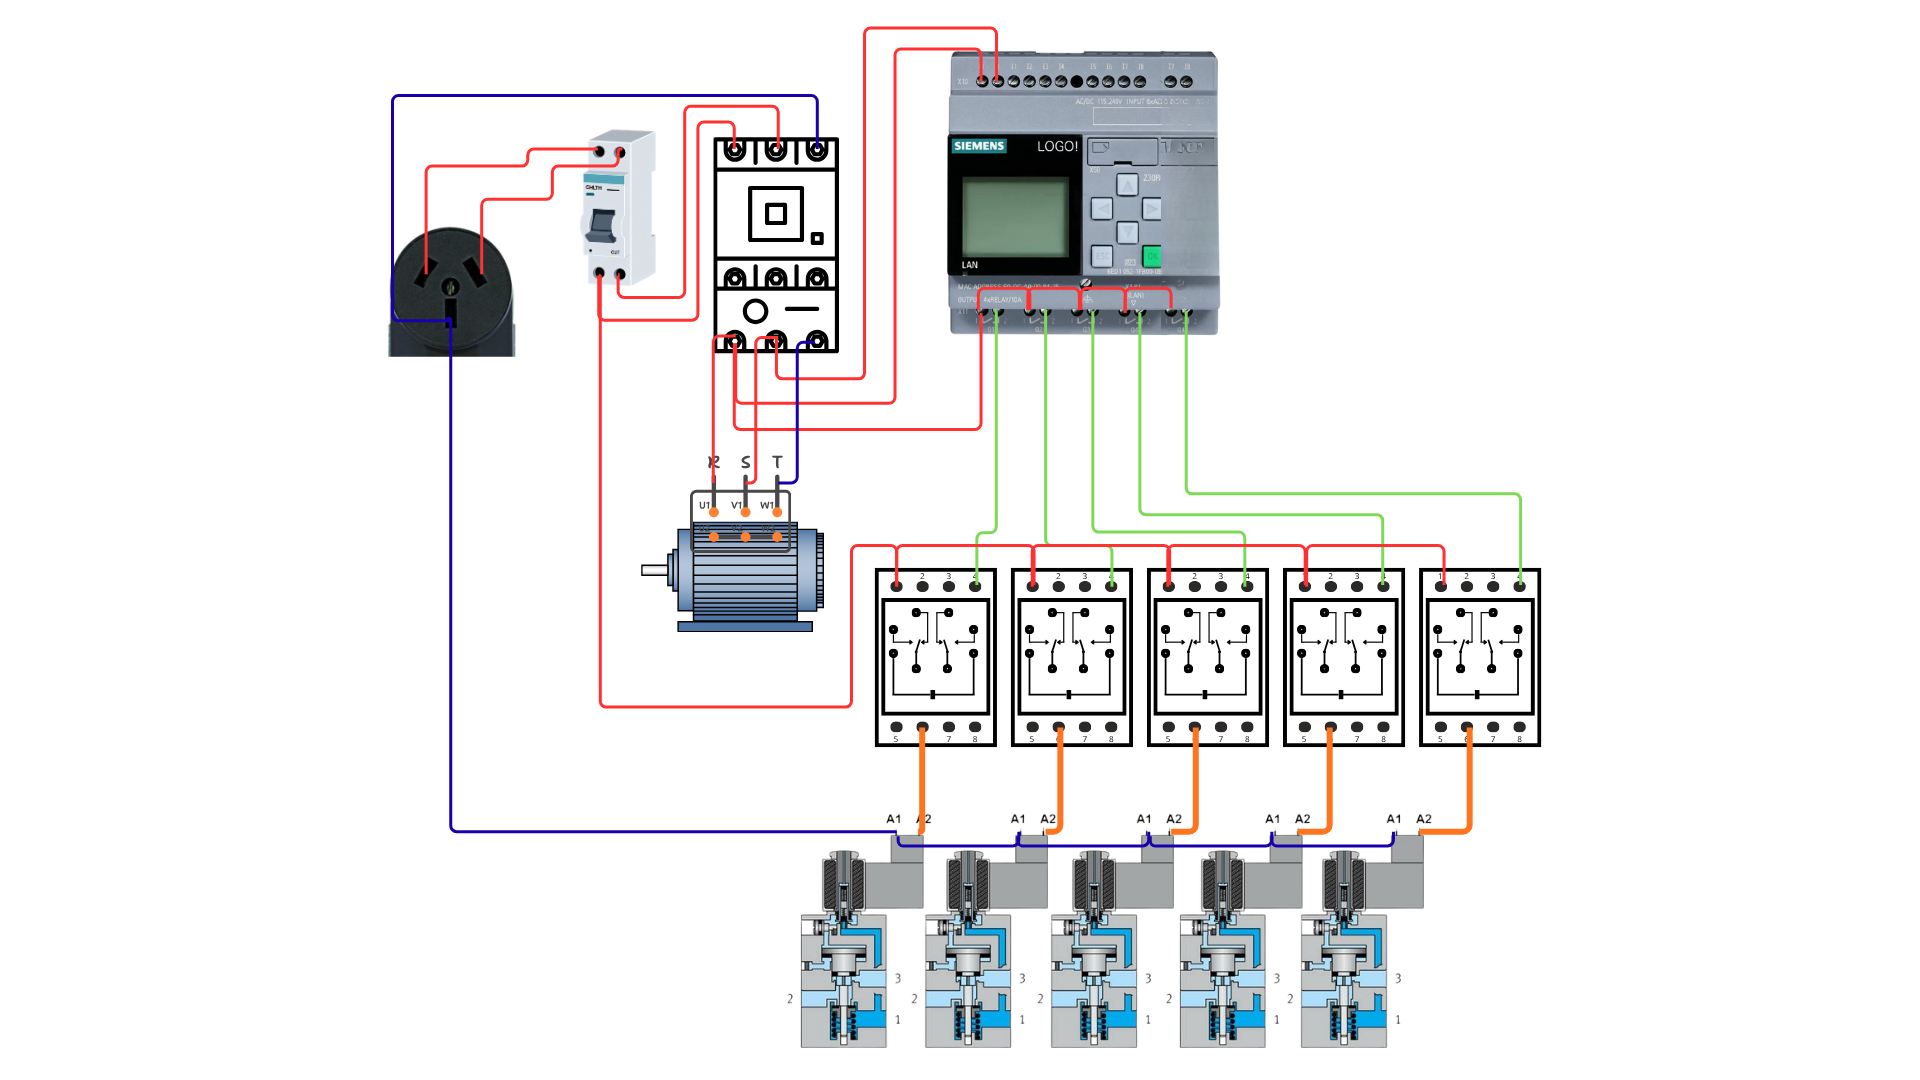
\includegraphics[width=0.80\textwidth]{Capítulos/fig/mapeo_señales.png}
\caption{Mapeo de señales originales, puntos de intervención y arquitectura de bypass.}
\label{fig:diag_diag}
\end{figure}

\section{Metodología de Desarrollo e Implementación}

Con el objetivo de alinear cada fase de diseño con su correspondiente validación técnica, se adoptó el modelo en V (\textit{V-Model}) adaptado a sistemas ciberfísicos. Esta metodología mitiga los riesgos de asincronía entre el modelo físico y su réplica virtual, garantizando que los requisitos sean verificados incrementalmente.

Las fases de ingeniería se estructuraron de la siguiente manera:

\begin{enumerate}
    \item \textbf{Fase 1 – Definición Arquitectónica.} Levantamiento del diagrama de estados original y definición de las capas ciberfísicas conforme a la familia de estándares ISO 23247 para gemelos digitales en manufactura. Se identificaron los flujos de información necesarios para el gemelo digital de nivel 3 (predictivo/interactivo), según la clasificación de madurez que establece la parte 2 de dicha norma \cite{iso23247-2}.
    
    \item \textbf{Fase 2 – Diseño de Subsistemas.} Modelado cinemático en Webots, programación de la máquina de estados finitos (FSM) en Python, diseño del SCADA en Node-RED y definición de los tópicos MQTT bajo el protocolo de mensajería ligera estandarizado por OASIS \cite{oasis2014}.
    
    \item \textbf{Fase 3 – Implementación Física.} Construcción del panel de control con grado de protección IP54, soldadura de la instrumentación aislada con optoacopladores, despliegue del broker Mosquitto y grabación del firmware en los dos microcontroladores ESP32.
    
    \item \textbf{Fase 4 – Verificación (Virtual Commissioning).} Ejecución de la FSM en Webots con inyección de perturbaciones y sincronización con los tópicos MQTT, utilizando la máscara de enrutamiento de Node-RED para aislar los comandos del hardware.
    
    \item \textbf{Fase 5 – Validación del Sistema.} Extracción de logs para el cálculo de latencias de red, tiempos de recuperación y la métrica de efectividad mecánica operativa (EMO) adaptada del OEE, conforme a los lineamientos de indicadores clave de desempeño de la ISO 22400 \cite{iso22400-2}.
\end{enumerate}

\begin{figure}[htbp]
\centering
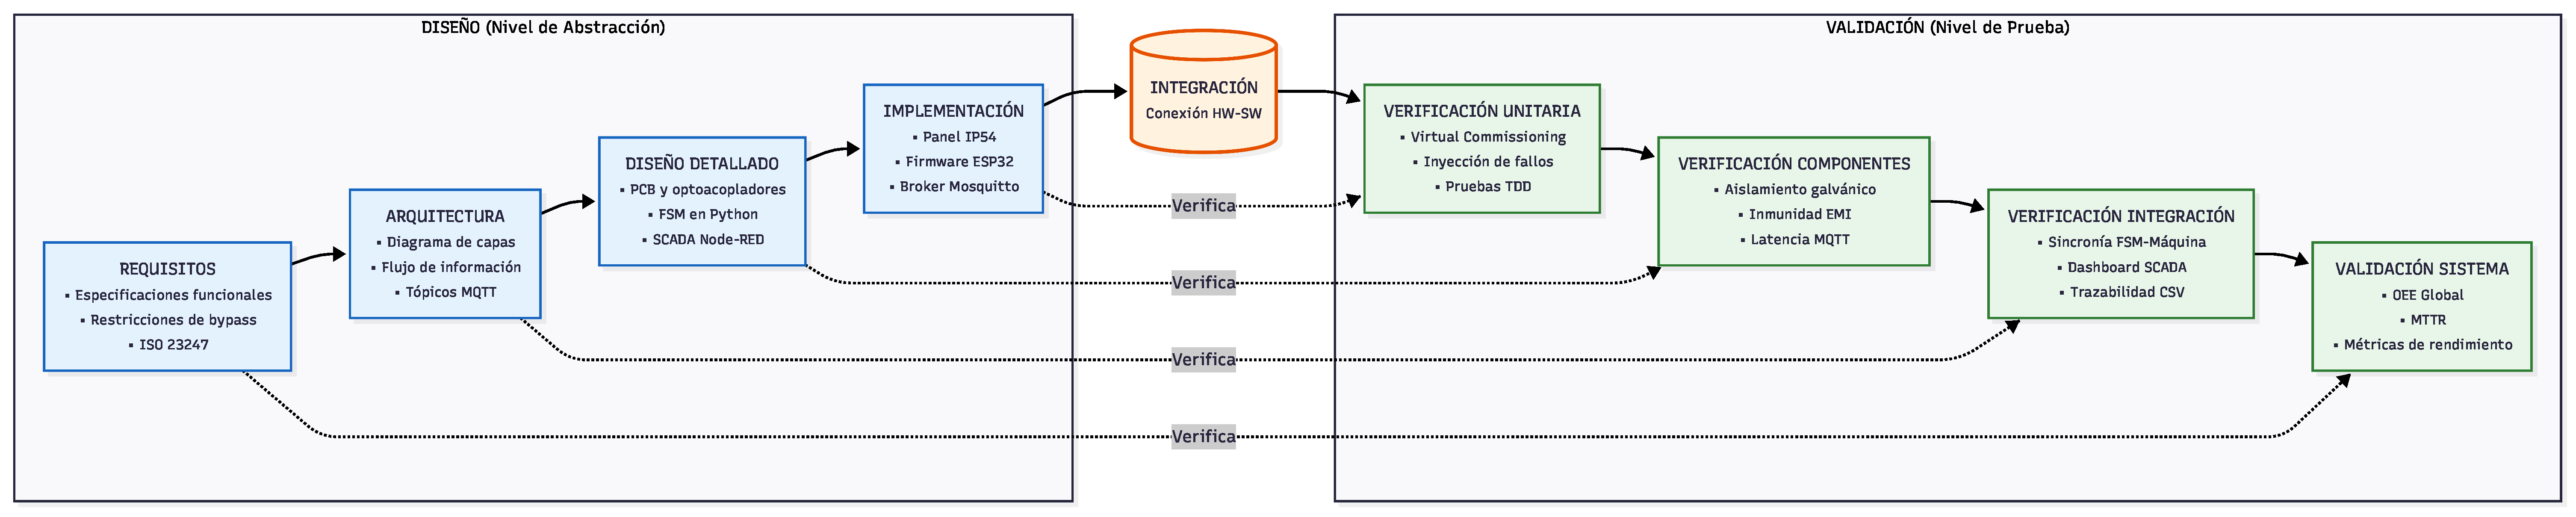
\includegraphics[width=0.9\textwidth, height=0.3\textheight, keepaspectratio=false]{Capítulos/img/V-MODEL.pdf}
\caption{Metodología V-Model aplicada al desarrollo del gemelo digital.}
\label{fig:diag_vmodel}
\end{figure}

\section{Técnicas e Instrumentos de Recolección de Información}

\subsection{Técnicas de Diagnóstico Físico}

La caracterización de la máquina legacy se sustentó en observación directa estructurada de los ciclos de dosificación y en el análisis de las señales eléctricas mediante un multímetro. Se realizó un mapeo completo de la secuencia electroneumática, registrando los tiempos de activación de las electroválvulas y el desplazamiento de los pistones con resolución de milisegundos. El uso de trazados de continuidad permitió identificar los puntos de bifurcación para el bypass sin alterar el cableado original, una práctica común en proyectos de retrofitting de maquinaria industrial \cite{retrofitting2025}.

\subsection{Instrumentos de Validación del Gemelo Digital}

El controlador de la FSM ejecutado en el entorno Webots genera un registro automático de transiciones de estado en archivos CSV con marcas de tiempo precisas. Durante las pruebas se almacenan, además de los cambios de estado, las latencias cinemáticas entre la orden enviada y la respuesta del actuador virtual. Estos datos constituyen la base para el cálculo posterior de la métrica EMO.

\subsection{Recolección de Telemetría MQTT}

La arquitectura de comunicación se fundamenta en una jerarquía estricta de tópicos. Los nodos ESP32 publican periódicamente las lecturas de los sensores bajo \texttt{maquina/sensor/\#} y los comandos de actuación fluyen por \texttt{maquina/actuador/\#}. Cada mensaje contiene un payload en formato JSON con los campos \texttt{timestamp}, \texttt{valor}, \texttt{unidad} y \texttt{calidad}. La frecuencia de muestreo se fijó en 100 ms para asegurar un sincronismo adecuado entre la planta física y el SCADA, aprovechando las características de baja latencia del protocolo MQTT \cite{oasis2014}.

\begin{figure}[htbp]
    \centering
%    \begin{minipage}{0.48\textwidth}
    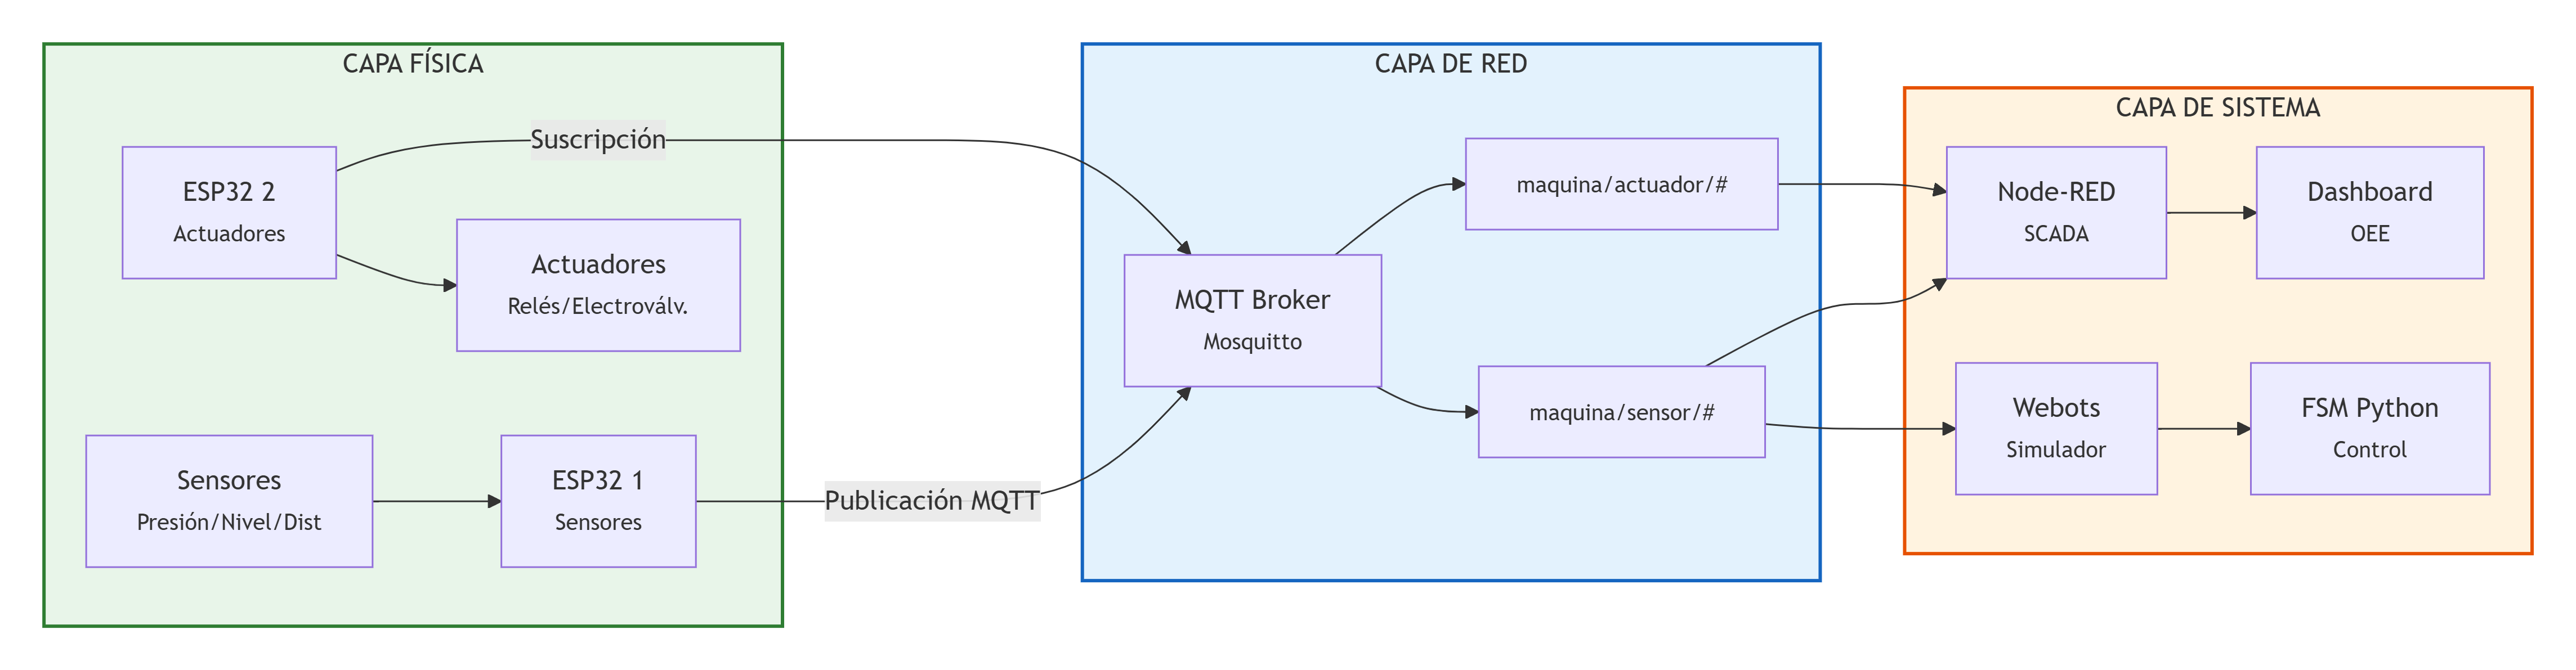
\includegraphics[width=0.9\textwidth, height=0.1\textheight, keepaspectratio=false]
    {Capítulos/img/flujomqtt.png}
    
\caption{Flujo completo de datos, formatos de payload y frecuencias de publicación.}
\label{fig:diag_flujo_info}
%\end{minipage}
\end{figure}

\section{Configuración e Implementación de Equipos}

\subsection{Configuración del ESP32 como Nodo de Borde}

Los dos microcontroladores ESP32-DevKit v1 (38 pines) fueron configurados con las siguientes asignaciones de pines:
\begin{itemize}
    \item Sensores infrarrojos (entrada digital con optoacoplador PC817) en GPIO 14, 15, 16.
    \item Sensor ultrasónico HC-SR04: Trig en GPIO 17, Echo en GPIO 18.
    \item Transductor de presión industrial 4-20 mA, leído a través de un conversor analógico-digital con filtro de promedio móvil de 10 muestras.
    \item Display TM1637 (I2C) y expansores de puertos PCF8574 para la interfaz HMI física.
    \item Cliente MQTT implementado con la librería \texttt{PubSubClient}; conexión WiFi con QoS 1 para los tópicos de estado y comandos.
\end{itemize}

Se implementaron filtros digitales de promedio móvil para suavizar las lecturas analógicas de presión y eliminar el ruido de alta frecuencia inducido por el contactor trifásico. La plataforma ESP32 fue seleccionada por su conectividad WiFi integrada, su arquitectura de doble núcleo que permite ejecutar simultáneamente la pila de comunicación MQTT y la lógica de control, y un costo reducido que la convierte en una opción idónea para nodos de borde en entornos IIoT \cite{espressif2023}.

\subsection{Configuración del Broker Mosquitto}

El broker MQTT se desplegó sobre un sistema operativo Linux en una máquina virtual dedicada. Se habilitaron los puertos 1883 (MQTT) y 9001 (WebSockets), y se aplicó autenticación básica (usuario/contraseña) para restringir accesos no autorizados. Se activó la persistencia de mensajes y la retención de estados (\textit{retained messages}) para que los suscriptores nuevos reciban de inmediato el último valor conocido de cada sensor, garantizando la consistencia del estado incluso después de desconexiones temporales.

\subsection{Configuración de Node-RED como SCADA}

Se instalaron los nodos adicionales para MQTT (entrada/salida), \texttt{Dashboard}, \texttt{JSON parser} y \texttt{SQLite}. Los flujos principales son:
\begin{itemize}
    \item Suscripción a los tópicos \texttt{maquina/sensor/\#} para visualización en tiempo real.
    \item Enrutamiento condicional: cuando el selector físico está en modo \textit{Simulación}, los comandos de actuador se publican bajo el prefijo \texttt{maquina/simulacion/actuador/\#}, que es leído exclusivamente por el controlador de Webots, aislándolo del hardware.
    \item Almacenamiento de los datos históricos en una base SQLite para el análisis post-prueba.
\end{itemize}

La elección de Node-RED responde a su modelo de programación visual, su conectividad nativa con MQTT y la capacidad de generar dashboards web de manera ágil, cualidades que han sido validadas en numerosos casos de uso de la Internet de las Cosas.

\subsection{Configuración de Webots como Simulador Ciberfísico}

Los modelos 3D generados en FreeCAD se importaron en formatos STL y OBJ. Los pistones se modelaron mediante nodos \texttt{SliderJoint} con dos posiciones discretas, y las trampillas con nodos \texttt{HingeJoint}. El controlador Supervisor, escrito en Python, ejecuta la FSM y utiliza el cliente Paho-MQTT para suscribirse y publicar en los tópicos correspondientes. La sincronización se logra a través de un lazo de control que, cada 100 ms, envía el estado actual del gemelo a \texttt{maquina/estado/fsm}.

Webots fue seleccionado por superar a otros simuladores en los criterios de integración con Python, bajo consumo de CPU y capacidad para modelar restricciones mecánicas discretas sin necesidad de motores físicos complejos \cite{michel2004}. La simulación no exige recursos de GPU elevados, lo que permite ejecutarla en el mismo equipo que aloja el SCADA y el broker MQTT durante las pruebas de laboratorio.

\begin{figure}[htbp]
\centering
    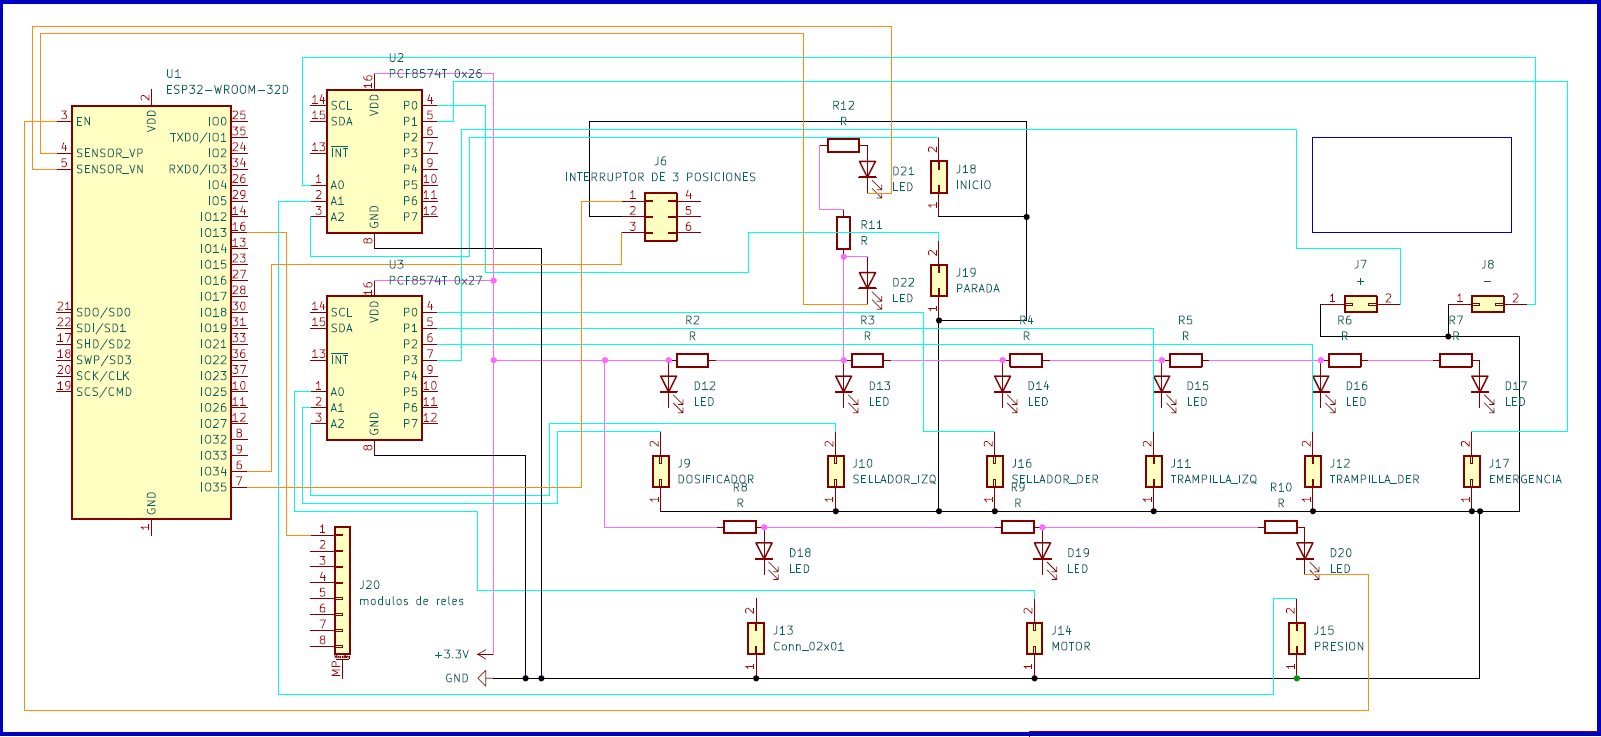
\includegraphics[width=1\textwidth]{Capítulos/img/DIAGRAMA ESQUEMATICODELPANELSCADA.png}
\caption{Esquemático del panel de control IP54.}
\label{fig:esq_panel}
\end{figure}

\begin{figure}[htbp]
\centering
    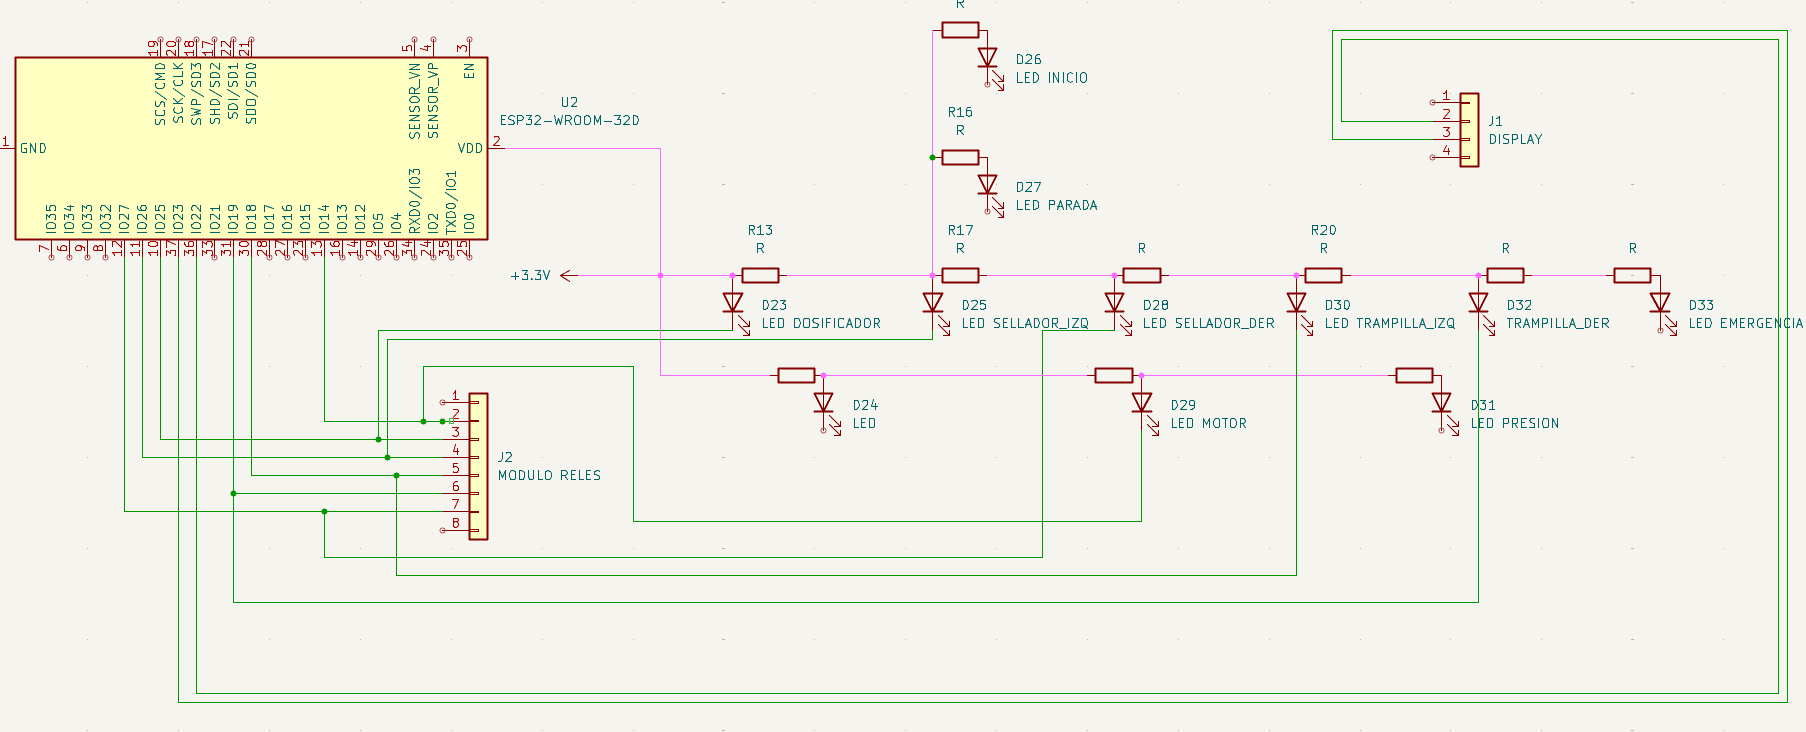
\includegraphics[width=1\textwidth]{Capítulos/img/DIAGRAMARELES.png}
\caption{Conexión de relés.}
\label{fig:conex_relays}
\end{figure}

\section{Requerimientos del Sistema}

\subsection{Requerimientos Funcionales}

\begin{enumerate}
    \item \textbf{RF1 – Control Híbrido y Bypass.} El panel físico instrumentado debe permitir la alternancia entre modo Manual (control unitario) y modo Automático, aislando estas rutinas de la lógica original del PLC mediante el banco de relés independientes.
    \item \textbf{RF2 – Enclavamiento de Seguridad (Interlocks).} El algoritmo de la FSM debe impedir la activación manual de cualquier actuador mientras el ciclo automático esté en ejecución.
    \item \textbf{RF3 – Fidelidad Cinemática en 3D.} El gemelo digital, desarrollado en Webots, debe emular los pistones neumáticos respetando exactamente sus dos posiciones discretas y las restricciones mecánicas de la máquina real.
    \item \textbf{RF4 – Secuestro de Señales (Aislamiento Virtual).} Node-RED debe interceptar las órdenes de control e inyectar el prefijo de simulación (e.g., \texttt{maquina/simulacion/actuador/piston}) cuando el selector de modo esté en Simulación, comandando únicamente al gemelo sin accionar el hardware físico.
    \item \textbf{RF5 – Telemetría en Tiempo Real.} El ESP32 debe publicar lecturas de los sensores cada 100 ms en los tópicos MQTT, indicando marca temporal y calidad del dato.
    \item \textbf{RF6 – Datalogging Automatizado.} El controlador de Webots y el flujo de Node-RED deben registrar transiciones de estado y eventos con timestamp, generando archivos CSV para el análisis posterior.
\end{enumerate}

\subsection{Requerimientos No Funcionales}

\begin{enumerate}
    \item \textbf{RNF1 – Latencia de Red.} El intercambio de mensajes a través del broker Mosquitto debe operar con una latencia inferior a 100 ms para mantener el sincronismo del SCADA.
    \item \textbf{RNF2 – Inmunidad al Ruido Eléctrico.} Todas las entradas digitales de los sensores deben estar aisladas galvánicamente mediante optoacopladores PC817, evitando reinicios del ESP32 por inducciones electromagnéticas del contactor trifásico.
    \item \textbf{RNF3 – Eficiencia Computacional.} El script de simulación en Webots debe ejecutarse de manera eficiente, sin saturar el procesador del equipo donde corre la simulación, permitiendo la operación en paralelo de otras tareas del sistema.
    \item \textbf{RNF4 – Disponibilidad del Broker.} Durante las pruebas de validación, el broker Mosquitto debe presentar una tasa de disponibilidad superior al 99.9\%.
    \item \textbf{RNF5 – Escalabilidad.} La arquitectura de tópicos MQTT debe permitir la adición de nuevos sensores o actuadores sin alterar la estructura base de nombres, facilitando futuras ampliaciones del gemelo digital.
\end{enumerate}

\section{Diseño de la Solución}
\label{sec:diseno_solucion}

\subsection{Diseño de Hardware (Capa Física)}

La etapa de entrada se protegió con optoacopladores PC817 que convierten las señales industriales de 12/24 V al nivel lógico de 3.3 V del ESP32, creando una barrera galvánica indispensable para la inmunidad al ruido. La alimentación de la caja de control se organizó en cascada: una fuente switching de 12 V/10 A y un módulo reductor Buck XL4015 a 5 V para los periféricos. El panel de control, alojado en una envolvente IP54, integra pulsadores mecánicos, un selector de tres posiciones, parada de emergencia y el display TM1637. El sensor de presión industrial con interfaz 4-20 mA se conectó a través de un filtro de promedio móvil implementado en firmware. Las salidas hacia actuadores se realizan mediante un módulo de relés de 8 canales, que replica las trayectorias de potencia del PLC original.

\subsection{Diseño de Red y Tópicos MQTT (Capa de Comunicación)}

Se definió una jerarquía estricta de tópicos MQTT:
\begin{itemize}
    \item \texttt{maquina/sensor/presion}
    \item \texttt{maquina/sensor/nivel\_tolva}
    \item \texttt{maquina/sensor/distancia}
    \item \texttt{maquina/actuador/electrovalvula}
    \item \texttt{maquina/actuador/piston}
    \item \texttt{maquina/simulacion/actuador/\#}
    \item \texttt{maquina/estado/fsm}
\end{itemize}

Los payloads se estructuran en JSON con los campos \texttt{timestamp} (ISO 8601), \texttt{valor} (numérico), \texttt{unidad} y \texttt{calidad} (0-100). Esta uniformidad facilita el procesamiento tanto en el SCADA como en el simulador.

\subsection{Diseño Cinemático Virtual (Capa de Software)}

El gemelo digital reproduce la volumetría real de la dosificadora a partir de modelos CAD exportados desde FreeCAD. En Webots se emplearon nodos \texttt{SliderJoint} para los pistones, con restricciones de posición que les permiten alcanzar solo dos estados (retraído/extendido), y nodos \texttt{HingeJoint} para las trampillas de dosificación. El controlador Supervisor, escrito en Python, ejecuta una FSM que refleja los estados del proceso y recibe comandos a través de MQTT.

\subsection{Ciclo de Vida de la Comunicación Ciberfísica}

El flujo de información inicia con la publicación periódica de telemetría desde el ESP32 al broker Mosquitto. Node-RED recibe, enriquece y enruta los datos hacia el dashboard SCADA y hacia el controlador de Webots. Los comandos generados por el operador o por la FSM viajan en sentido inverso: Node-RED decide, según el modo de operación, si se envían al hardware real o únicamente al gemelo bajo el prefijo de simulación. Finalmente, el estado del sistema se registra tanto en la base de datos SQLite como en los archivos CSV del Supervisor.

\begin{figure}[htbp]
\centering    
%\begin{minipage}{0.48\textwidth}
    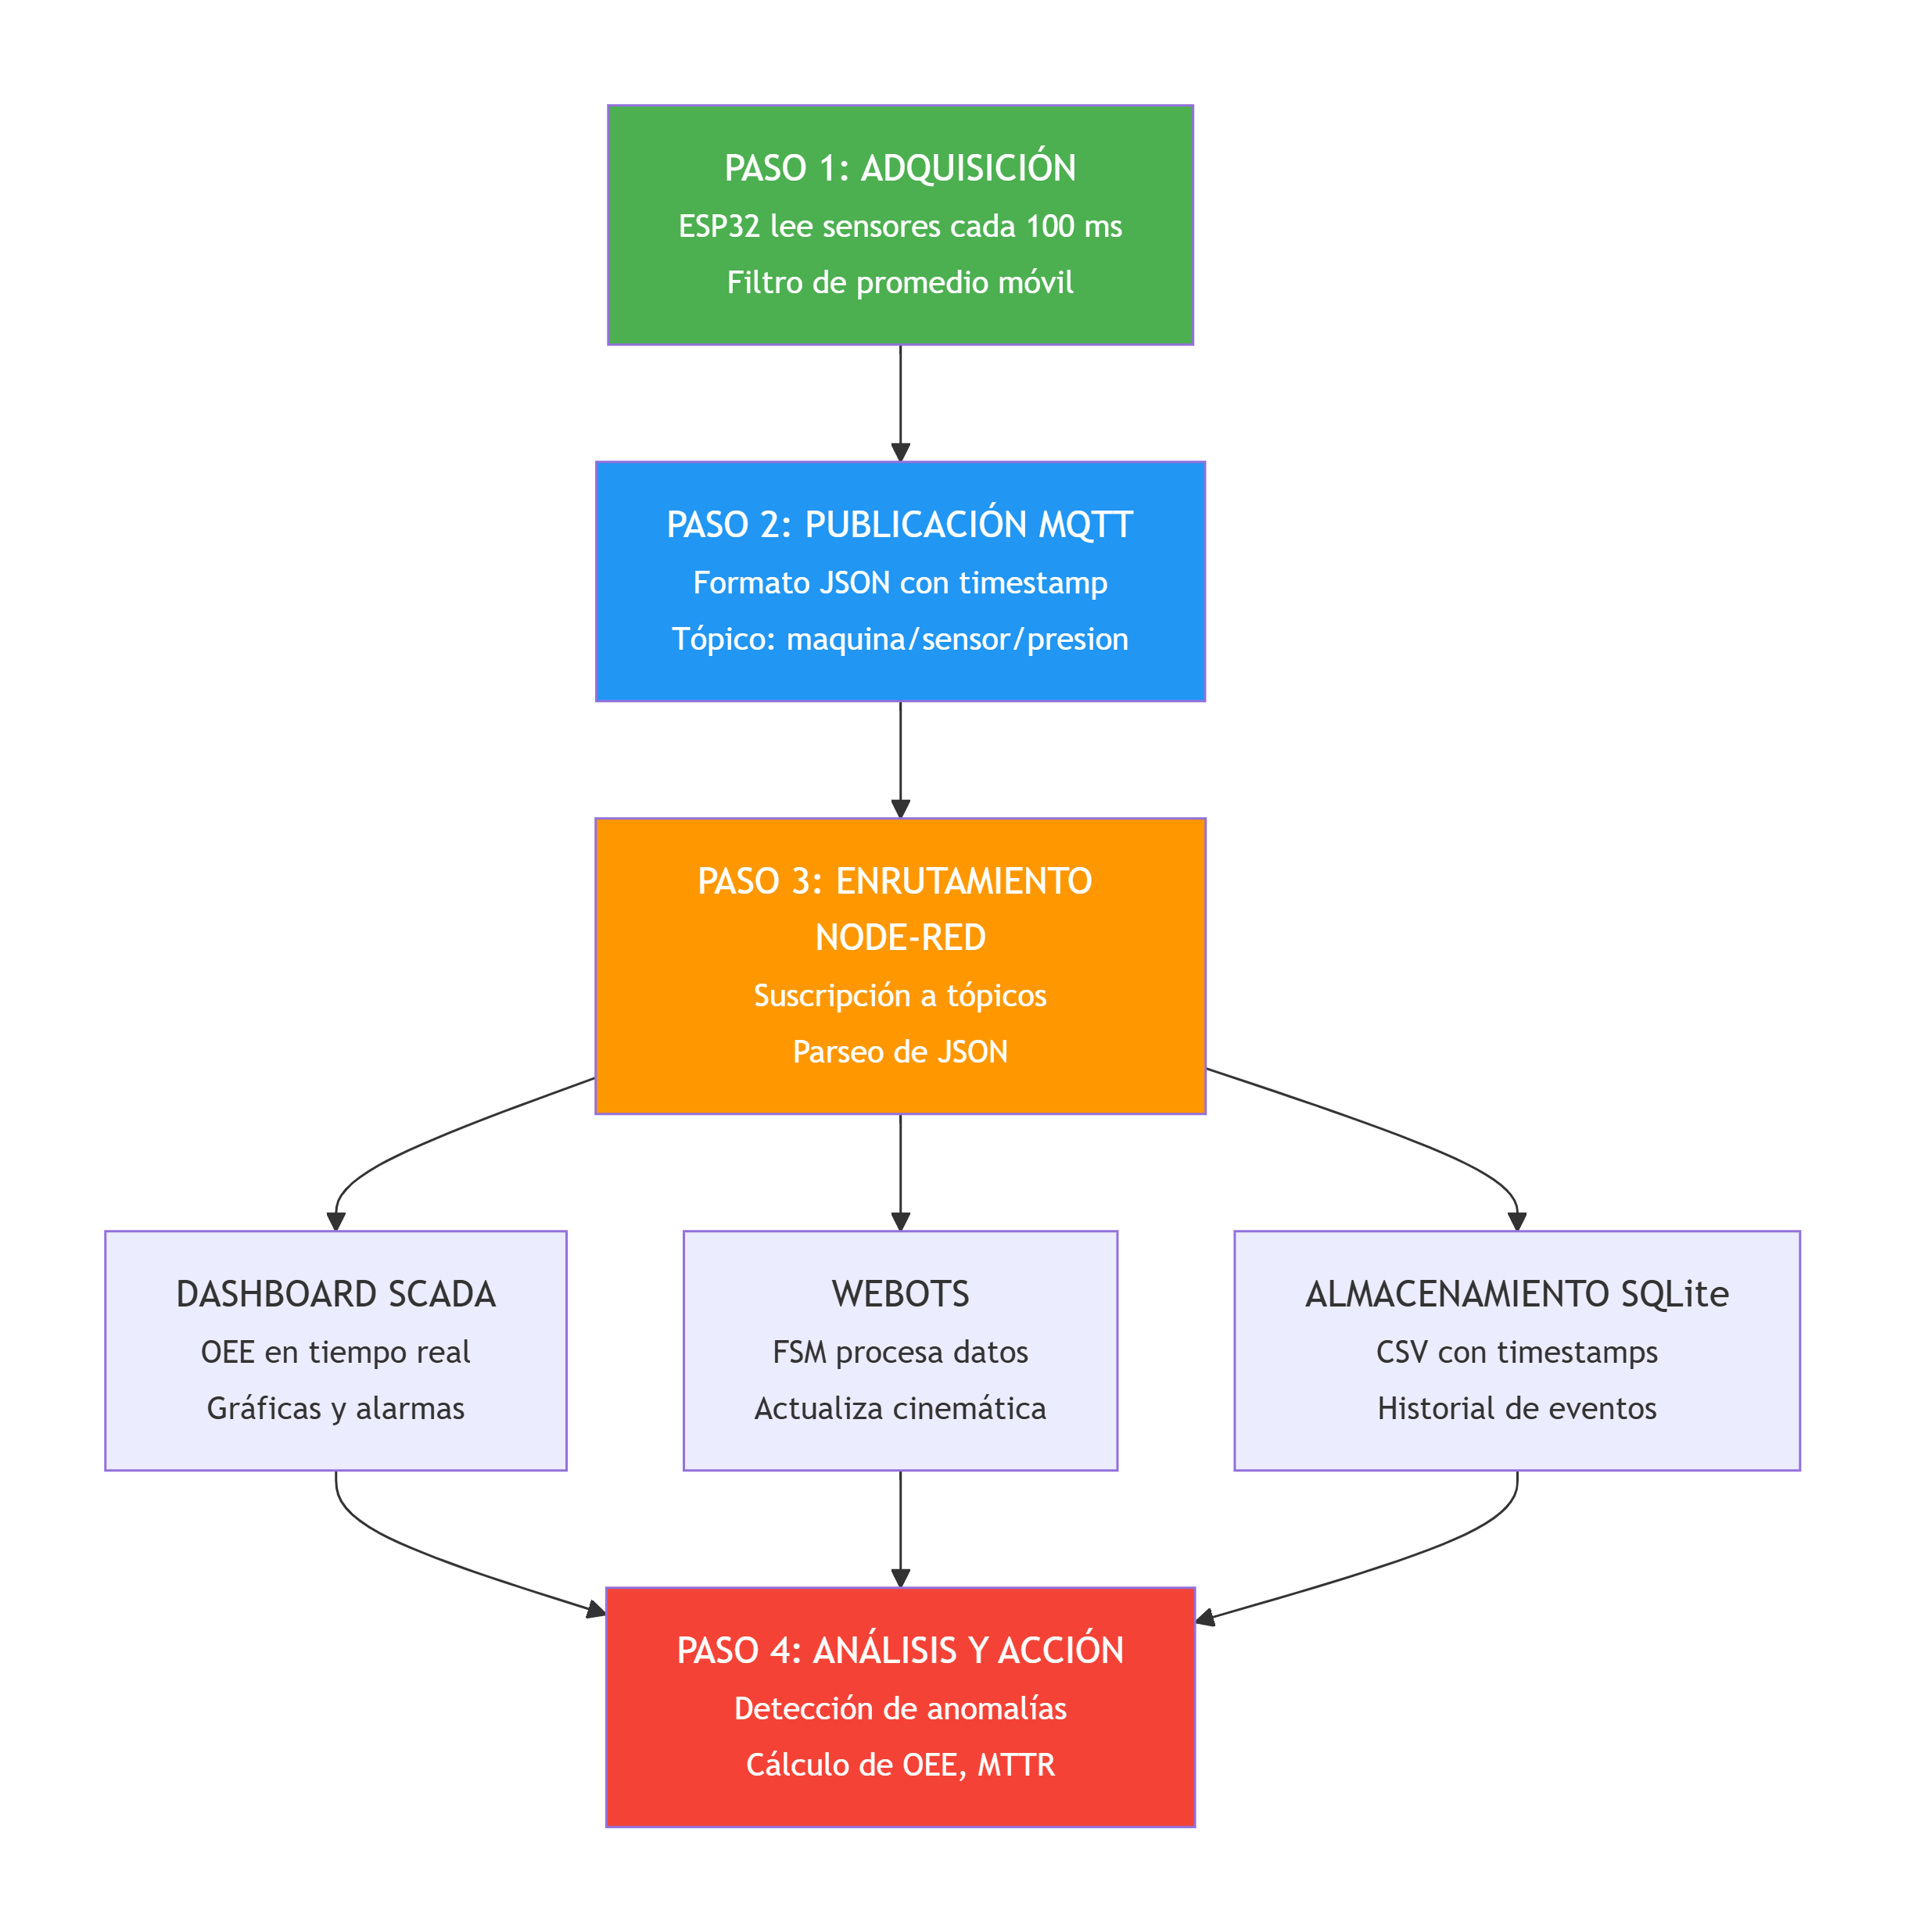
\includegraphics[width=0.9\textwidth]{Capítulos/img/ciclodevidacomunicacion.png}
\caption{Ciclo completo de la información desde el sensor hasta el registro histórico.}
\label{fig:ciclo_info}
%\end{minipage}
\end{figure}

\begin{figure}[htbp]
\centering
\begin{minipage}{0.48\textwidth}
    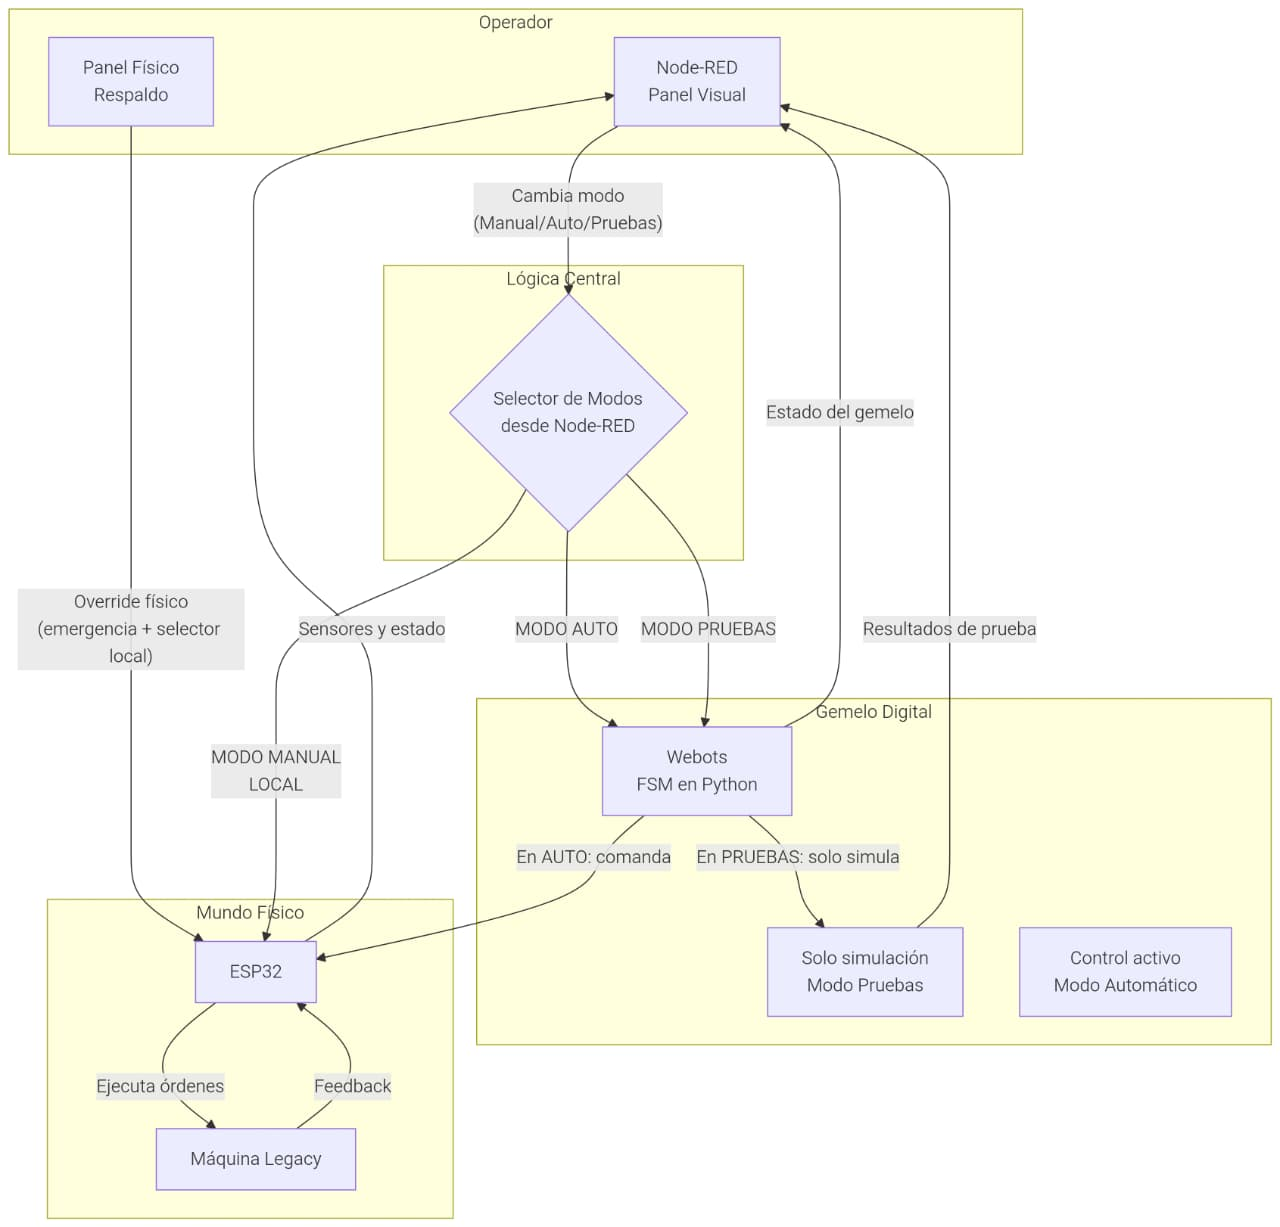
\includegraphics[width=0.9\textwidth]{Capítulos/img/arquitectura_sistema.jpeg}
\caption{Arquitectura global del gemelo digital implementado.}
\label{fig:arq_general}
\end{minipage}

\end{figure}

\subsection{Validación Geométrica del Modelo}

Para garantizar que el gemelo digital mantuviera una correspondencia volumétrica exacta, se compararon las dimensiones reales de la máquina con las del modelo importado en Webots. La Tabla~\ref{tab:comp_geom} muestra la coincidencia en distancias y posiciones de los actuadores, con una desviación máxima de 2 mm. Esta precisión es suficiente para que las restricciones cinemáticas y las colisiones se reproduzcan fielmente.

\begin{table}[htbp]
\centering
\caption{Comparación de dimensiones y posiciones geométricas.}
\label{tab:comp_geom}
\begin{tabular}{lcc}
\hline
\textbf{Parámetro} & \textbf{Valor real (mm)} & \textbf{Valor en Webots (mm)} \\
\hline
Carrera del pistón A & 80 & 80 \\
Carrera del pistón B & 120 & 120 \\
Diámetro de válvula & 35 & 35 \\
\hline
\end{tabular}
\end{table}

\section{Justificación Técnica y Adaptación de Métricas}

\subsection{Selección Tecnológica}

La elección del ESP32 frente a otras plataformas (Arduino, Raspberry Pi) se fundamenta en su conectividad WiFi integrada, su arquitectura dual-core (que permite manejar la comunicación MQTT y la lógica de control en paralelo) y su bajo costo, convirtiéndolo en la opción idónea para el nodo de borde del sistema ciberfísico \cite{espressif2023}. MQTT fue seleccionado sobre HTTP por su menor sobrecarga de cabeceras, su modelo de publicación/suscripción asíncrono y su amplia adopción en entornos IIoT, tal como lo respalda el estándar OASIS \cite{oasis2014}. Webots se impuso a otros simuladores (Nvidia Isaac Sim, Gazebo, Unity) por su integración nativa con Python, su bajo consumo de CPU y su capacidad para modelar restricciones mecánicas discretas sin necesidad de motores físicos complejos, características que lo consolidan como un entorno de simulación profesional para robótica y automatización \cite{michel2004}. Por último, Node-RED se prefirió a un SCADA tradicional por su entorno de programación visual, su conectividad MQTT nativa y la posibilidad de desplegar dashboards web de manera ágil, funcionalidades que han sido validadas en aplicaciones de IoT industrial.

\subsection{Adaptación de Métricas}

La métrica de referencia en la industria es la Efectividad Global del Equipo (OEE, por sus siglas en inglés), definida como el producto de la disponibilidad, el rendimiento y la calidad según la norma ISO 22400-2 \cite{iso22400-2}. La literatura especializada señala que el OEE es una herramienta clave para medir el desempeño de los equipos de manufactura \cite{muchiri2008}. Dado que en este proyecto no se dispone de celdas de carga ni de sistemas de visión artificial para medir la calidad del producto dosificado, se adaptó el OEE eliminando el factor de calidad, obteniendo así la \textbf{Efectividad Mecánica Operativa (EMO)}:

\begin{equation}
    \text{EMO} (\%) = \text{Disponibilidad} \times \text{Rendimiento} \times 100.
    \label{eq:emo}
    \addeqtolist{EMO: Efectividad Mecánica Operativa}
\end{equation}

Adicionalmente, se calculó el Tiempo Medio de Recuperación (\textit{Mean Time To Repair}, MTTR) ante fallos inyectados durante la fase de verificación:

\begin{equation}
    \text{MTTR} = \frac{\sum_{i=1}^{N} \text{tiempo de inactividad}_i}{N}.
    \label{eq:mttr}
    \addeqtolist{MTTR: Tiempo Medio de Recuperación}
\end{equation}

donde \(N\) es el número de eventos de fallo inducidos.

Los filtros de promedio móvil aplicados a la señal de presión siguen la ecuación:

\begin{equation}
    \overline{p}_k = \frac{1}{M} \sum_{i=0}^{M-1} p_{k-i}.
    \label{eq:presion}
    \addeqtolist{Filtro de promedio móvil para presión}
\end{equation}

con \(M=10\) muestras, suficiente para atenuar el ruido de conmutación del contactor sin introducir un retardo excesivo.

\section{Presupuesto y Recursos Económicos}

La inversión total necesaria para la implementación del bypass, la instrumentación y los nodos de comunicación se desglosa en la Tabla~\ref{tab:presupuesto}. Los precios corresponden a valores de mercado locales, y se incluye una partida para herramientas de laboratorio considerando una depreciación del 50\% de su vida útil.

\begin{longtable}{|p{6.5cm}|c|p{2cm}|c|}
\caption{Presupuesto detallado del proyecto.}
\label{tab:presupuesto}
\\\hline
\textbf{Componente/Herramienta} & \textbf{Cantidad} & \textbf{Precio Unitario (USD)} & \textbf{Subtotal (USD)} \\
\hline
\endfirsthead
\hline
\textbf{Componente/Herramienta} & \textbf{Cantidad} & \textbf{Precio Unitario (USD)} & \textbf{Subtotal (USD)} \\
\hline
\endhead
\hline
\endlastfoot
ESP32 DevKit v1 (38 pines) & 2 & 6.50 & 13.00 \\
Optoacopladores PC817 & 10 & 0.30 & 3.00 \\
Sensor de presión industrial 4-20 mA & 1 & 65.00 & 65.00 \\
Válvula reguladora de presión & 1 & 45.00 & 45.00 \\
Módulo relé 8 canales 5 V/10 A & 1 & 8.50 & 8.50 \\
Fuente switching 12 V/10 A & 1 & 22.00 & 22.00 \\
Módulo Buck XL4015 & 1 & 3.50 & 3.50 \\
Display TM1637 & 1 & 2.80 & 2.80 \\
Caja electrónica IP54 & 1 & 18.00 & 18.00 \\
Selector 3 posiciones & 1 & 4.00 & 4.00 \\
Botones pulsadores industriales & 12 & 1.20 & 14.40 \\
Cables jumper, AWG, conectores & Global & 15.00 & 15.00 \\
Kit de soldadura y herramientas & Global & 30.00 & 30.00 \\
\hline
\textbf{TOTAL} & & & \textbf{243.20} \\
\hline
\end{longtable}
% ==========================================================
% CAPÍTULO III
% ==========================================================
\input{Capítulos/03_Implementación}
% ==========================================================
% CAPÍTULO IV
% ==========================================================
\chapter{Conclusiones y Recomendaciones}
\label{chap:conclusiones}

\section{Conclusiones}

\subsection{Validación del Objetivo General y la Hipótesis Ciberfísica}

En el contexto de la presente investigación, hemos logrado demostrar empíricamente la viabilidad técnica y la validez funcional de implementar un Gemelo Digital de Nivel 3 con capacidades predictivas e interactivas sobre una máquina dosificadora de granos de naturaleza \textit{legacy}. Nuestra hipótesis fundamental del proyecto sostenía que era posible modernizar un equipo industrial obsoleto sin alterar su arquitectura electromecánica original mediante un \textit{bypass} ciberfísico no intrusivo. Los resultados cuantitativos que obtuvimos durante las jornadas de validación experimental en el Laboratorio de Procesos confirman esta premisa. Mediante la integración efectiva que realizamos de los tres pilares del sistema el \textit{hardware} de instrumentación externa basado en controladores ESP32, el \textit{middleware} de comunicación soportado por el protocolo MQTT y el broker Mosquitto, y el entorno de simulación 3D en Webots logramos constituir un sistema ciberfísico cohesivo.

La evidencia más contundente del cumplimiento de nuestro objetivo general reside en que conseguimos una Efectividad General de los Equipos (OEE) promedio del 91.85\% con una desviación estándar de apenas $\pm 0.46\%$ durante los ciclos operativos normales. Con esta métrica, complementada por una Disponibilidad del 100\% y un Rendimiento equivalente fuera de los escenarios de fallo, demostramos que el gemelo digital no solo funciona como un espejo pasivo del proceso físico, sino que mantiene la estabilidad y eficiencia del sistema. Validamos de manera crítica la capacidad predictiva, característica distintiva del Nivel 3 en la pirámide de los gemelos digitales, en la Prueba 5. En dicho escenario, inyectamos un fallo en el sistema neumático que el modelo virtual detectó y reflejó, lo cual nos permitió una reacción asistida como operadores que resultó en un Tiempo Medio de Reparación (MTTR) de 52 segundos y una disponibilidad durante el evento de fallo del 92.92\%. Con estos valores confirmamos que el gemelo digital trasciende la mera monitorización para convertirse en una herramienta de apoyo a la decisión en tiempo real.

\subsection{Cumplimiento de los Objetivos Específicos y Ejecución Metodológica}

Guiamos el desarrollo del proyecto mediante un marco metodológico estructurado que desglosamos en tres objetivos específicos; alcanzamos cada uno de ellos a cabalidad y contribuimos de manera sinérgica al éxito de nuestro prototipo final.

En primer lugar, cumplimos el objetivo específico OE1 (Levantamiento y diagnóstico) mediante un proceso exhaustivo de ingeniería inversa que llevamos a cabo. Ante la falta de documentación técnica actualizada del equipo \textit{legacy}, realizamos un mapeo detallado del circuito eléctrico a 220V y de la lógica de control original gobernada por un PLC. Este diagnóstico nos permitió identificar el punto exacto de intervención en la entrada 1 del PLC, proveniente del contactor trifásico, lo cual fue fundamental para que diseñáramos el \textit{bypass} sin desencadenar conflictos lógicos ni riesgos eléctricos. La instalación de la sensórica (infrarrojos, ultrasónico y transductor de presión) que efectuamos respondió directamente a nuestra necesidad de caracterizar el comportamiento neumático y mecánico previamente oculto.

En segundo lugar, concretamos el objetivo OE2 (Diseño e implementación) con la materialización completa de la arquitectura que propusimos. Diseñamos el \textit{hardware} de la caja de control externa, resolviendo las limitaciones de pines de los ESP32 mediante módulos de expansión I2C y mitigando las interferencias electromagnéticas con un condensador de poliéster dimensionado para la carga inductiva de los contactores. Paralelamente, desarrollamos la arquitectura de \textit{software}, implementando la Máquina de Estados Finitos (FSM) en Python dentro de Webots y programando los nodos de comunicación y el SCADA en Node-RED. Al hacer converger ambos desarrollos, logramos una latencia de comunicación MQTT promedio de 0.61 ms, un valor excepcionalmente por debajo del umbral de 100 ms que establecimos en los requerimientos no funcionales, garantizando así una sincronía efectiva entre el mundo físico y el virtual.

Finalmente, acometimos el objetivo OE3 (Evaluación) mediante un riguroso plan de pruebas en el que procesamos lotes de producción desde 60 hasta 200 fundas. En esta fase no nos limitamos a verificar la funcionalidad, sino que generamos un conjunto de datos cuantitativos robustos. Con la repetibilidad de la métrica OEE en las cuatro pruebas sin fallo, con una variación mínima, validamos la consistencia de nuestra instrumentación y la robustez del algoritmo de control. Al ejecutar completamente el proyecto dentro de un presupuesto de \$243.20 USD, validamos que alcanzamos los objetivos técnicos bajo estrictas restricciones económicas, maximizando la relación costo-beneficio.

\subsection{Aportaciones Técnicas al Campo de los Sistemas Ciberfísicos y la Manufactura}

Más allá de la solución puntual, con este trabajo dejamos un legado de aportaciones técnicas y metodológicas relevantes para la Ingeniería en Tecnologías de la Información. Nuestra principal contribución es que formalizamos una metodología de \textit{bypass} ciberfísico no intrusivo para la modernización de máquinas \textit{legacy}. A diferencia de un \textit{retrofit} tradicional que requiere la modificación completa del tablero de control, nuestro enfoque nos permite instrumentar externamente el proceso, preservando la integridad del circuito original de 220V y la lógica del PLC. Con esta metodología minimizamos el riesgo de inutilizar equipos críticos cuya detención prolongada no es viable.

En segundo lugar, hemos validado una arquitectura de integración vertical de bajo costo que desafía el paradigma de que los gemelos digitales requieren plataformas comerciales de alto valor. Utilizando microcontroladores ESP32 de amplia disponibilidad, protocolos ligeros como MQTT y plataformas de simulación de código abierto como Webots, logramos un sistema plenamente funcional descrito en detalle teórico y práctico. Constituimos este proyecto como un caso de estudio replicable y totalmente documentado para entornos académicos y de formación técnica, con el cual proporcionamos un manual para la transformación digital de laboratorios universitarios. En el ámbito de la interoperabilidad, hemos demostrado cómo un protocolo IoT moderno puede inyectar datos de un activo \textit{legacy} en un ecosistema digital, un paso fundamental para la Industria 4.0.

\subsection{Identificación de Limitaciones y Restricciones del Prototipo Actual}

Consideramos imperativo para el rigor científico reconocer las limitaciones que enmarcaron el alcance de nuestro proyecto. Nuestra restricción más significativa fue la imposibilidad de medir la Calidad dentro del indicador OEE. La ausencia de un sistema de pesaje dinámico (celdas de carga) o de un subsistema de visión artificial en la etapa de dosificación nos impidió cuantificar la precisión en gramos de cada funda. Por lo tanto, el OEE que reportamos (91.85\%) es una métrica compuesta únicamente por Disponibilidad y Rendimiento, lo cual consideramos que subestima potencialmente las pérdidas del proceso si existiesen variaciones no detectadas en la masa del producto. Enfrentamos esta realidad como consecuencia directa de la naturaleza \textit{legacy} de la máquina y de la falta de permisos que tuvimos para modificar su tolva de pesaje original.

En segundo lugar, circunscribimos el dominio de validación a un entorno controlado de laboratorio. Si bien esto fue adecuado, reconocemos que las condiciones no replican completamente las perturbaciones ambientales de una planta agroindustrial real, como el polvo en suspensión, las fluctuaciones extremas de temperatura o las vibraciones constantes transmitidas por otras máquinas. Asimismo, el único escenario de fallo inyectado que probamos fue la desconexión del sistema neumático, un modo de fallo común pero no el único posible en el sistema electromecánico completo. Finalmente, en nuestra implementación no estuvimos exentos de desafíos en la gestión del cronograma. En la fase de integración entre la Máquina de Estados Finitos (FSM) y el entorno de simulación Webots, enfrentamos una curva de aprendizaje más pronunciada de lo que estimamos, lo cual reflejamos en una extensión justificada de 3 días en nuestro plan de trabajo original.

\subsection{Reflexión Final Sobre la Transformación Digital de Activos Industriales}

Al término de esta investigación, reflexionamos sobre el impacto de la transformación digital en el tejido industrial latinoamericano. Hemos constatado que la obsolescencia tecnológica no es un destino irreversible, sino un estado transitorio que logramos resolver mediante inteligencia ciberfísica. Con nuestro proyecto demostramos que la ecuación de modernización no se limita a la disyuntiva del reemplazo de equipos, sino que se enriquece con una tercera vía: la \enquote{digitalización envolvente}. Este enfoque que proponemos permite a las pequeñas y medianas empresas, que conforman la mayor parte del sector agroindustrial, acceder a las ventajas de la Industria 4.0 sin ejecutar inversiones prohibitivas. Comprobamos que la combinación estratégica de talento humano en formación de pregrado y herramientas tecnológicas de código abierto tiene el poder de catalizar un cambio profundo en la competitividad del sector productivo.

\section{Recomendaciones}

A la luz de los resultados que obtuvimos, las lecciones que aprendimos y la prospectiva tecnológica, presentamos las siguientes recomendaciones estructuradas para los diferentes actores involucrados, con el fin de maximizar el impacto y la sostenibilidad de nuestra solución.

\subsection{Recomendaciones para el Laboratorio de Procesos de la Universidad Indoamérica}

Instamos a los responsables del Laboratorio de Procesos a incorporar formalmente el Gemelo Digital que desarrollamos como un módulo didáctico transversal. Consideramos que esta herramienta no debe limitarse a una demostración, sino convertirse en un banco de pruebas para asignaturas de automatización industrial, sistemas ciberfísicos y protocolos de comunicación. Recomendamos diseñar guías de laboratorio específicas donde los estudiantes utilicen el SCADA de Node-RED para analizar tendencias de rendimiento y simular fallos, fortaleciendo así sus competencias en diagnóstico de fallos.

Asimismo, sugerimos establecer un protocolo de mantenimiento predictivo básico aprovechando las métricas que recolectamos. Aunque el sistema actual no prescribe acciones automáticas, el personal del laboratorio puede utilizar nuestros datos de presión del sistema neumático monitoreado en tiempo real para anticipar ciclos de mantenimiento antes de que ocurra una caída de presión crítica. Para enriquecer el ecosistema de sensórica, recomendamos la adquisición de sensores adicionales de vibración y temperatura que puedan integrarse a los pines de expansión I2C que actualmente usamos, mejorando así la riqueza informativa del gemelo sin alterar la arquitectura base.

\subsection{Recomendaciones para la Universidad Indoamérica y la Gestión Curricular}

Desde la perspectiva institucional, recomendamos a la Universidad Indoamérica establecer un laboratorio especializado en Gemelos Digitales y Sistemas Ciberfísicos. La exitosa ejecución que logramos en este proyecto con un presupuesto tan austero establece un precedente para equipar un espacio dedicado con múltiples máquinas \textit{legacy} instrumentadas. Este laboratorio posicionaría a la universidad como un referente en la enseñanza de TIC aplicadas a la industria. Consideramos crucial fomentar proyectos de titulación que sigan esta línea de investigación aplicada, cerrando la brecha entre la teoría académica y las necesidades tangibles de la industria local.

Recomendamos a las autoridades académicas gestionar alianzas estratégicas con el sector agroindustrial de la provincia. Esta transferencia tecnológica directa nos permitiría calibrar el prototipo en condiciones reales y, al mismo tiempo, ofrecer a los empresarios una ventana de oportunidad para la modernización de bajo riesgo. La inclusión de contenidos sobre protocolos IoT industriales (MQTT, OPC UA) y simulación 3D en la actualización curricular de la Ingeniería en Tecnologías de la Información es igualmente prioritaria para que garanticemos que los futuros ingenieros dominen estas competencias clave.

\subsection{Recomendaciones Estratégicas para el Sector Agroindustrial}

Para las empresas del sector agroindustrial, ofrecemos con este proyecto un modelo de adopción tecnológica de bajo riesgo. Nuestra recomendación principal es realizar un análisis de costo-beneficio que compare el \textit{bypass} ciberfísico que presentamos aquí con la compra de una máquina nueva equivalente. Nuestros resultados indican que, por menos de 250 dólares, logramos que una empresa transite de una operación operativamente \enquote{ciega} a un modelo con monitorización en tiempo real, lo cual impacta directamente en los indicadores de disponibilidad.

Recomendamos a los gerentes de planta considerar la monitorización del OEE, incluso sin el factor de calidad automático, como un primer paso para implementar la Mejora Continua. La visibilidad que otorgamos con el tablero SCADA sobre los tiempos de ciclo y los micro-paros le permite al supervisor identificar cuellos de botella invisibles a simple vista. La gran ventaja de nuestro enfoque es que nos apoyamos en tecnología \textit{open-source}, lo cual elimina los costos de licenciamiento de software propietario, reduciendo dramáticamente las barreras de entrada para pequeñas y medianas empresas procesadoras.

\subsection{Recomendaciones Técnicas para Iteraciones Futuras del Hardware y Software}

Técnicamente, recomendamos que en la próxima iteración del prototipo se priorice la incorporación del factor de Calidad en el cálculo del OEE. Podemos lograr esto mediante la integración de una celda de carga y un módulo conversor analógico-digital de alta precisión, que añadiremos al bus I2C existente, para registrar el peso exacto de cada funda. Paralelamente, sugerimos el desarrollo de una aplicación móvil o una interfaz web responsive que actúe como cliente del broker MQTT, lo que nos permitirá el monitoreo remoto de la producción desde cualquier dispositivo.

Para mejorar la resiliencia del sistema embebido, aconsejamos implementar la lógica de \textit{watchdog} en los ESP32 para reinicios automáticos en caso de bloqueo del firmware. Además, consideramos que debemos expandir nuestro modelo de la Máquina de Estados Finitos (FSM) actual, que contempla un escenario de falla neumática, para incluir estados correspondientes a fallas eléctricas, atascos de granos o desconexión del bus de comunicación. Finalmente, aunque el consumo que logramos es abordable, mediante una auditoría energética del sistema implementado podríamos optimizar los ciclos de sueño profundo de los microcontroladores, una ventaja crucial si decidiéramos desplegar el sistema en ubicaciones con suministro eléctrico inestable.

\section{Trabajos Futuros}

Con la culminación de nuestro proyecto no cerramos el ciclo de investigación, sino que abrimos un abanico de líneas de trabajo futuras que se alinean con la evolución natural de los gemelos digitales y la ingeniería de sistemas ciberfísicos.

\subsection{Evolución hacia un Gemelo Digital Prescriptivo (Nivel 4)}

La línea de investigación más directa que abrimos es la migración de nuestro actual gemelo de Nivel 3 (Predictivo) a uno de Nivel 4 (Prescriptivo). Esto implica que diseñemos e integremos algoritmos de inteligencia artificial que no solo anticipen el fallo, sino que recomienden autónomamente la acción correctiva. Proponemos explorar el uso de redes neuronales artificiales para modelar el desgaste de los pistones neumáticos basándonos en la data histórica de presión que recolectamos. Del mismo modo, podríamos optimizar en tiempo real la cadencia de los actuadores mediante la implementación de algoritmos genéticos para maximizar el OEE sujeto a restricciones de fatiga de materiales, logrando así transitar de la alerta a la decisión autónoma.

\subsection{Nuevas Líneas de Investigación Aplicada en Ciberfísica}

Recomendamos la derivación de este trabajo hacia la aplicación de nuestra metodología de \textit{bypass} en otras familias de máquinas \textit{legacy} presentes en los talleres de la universidad, como tornos paralelos, fresadoras convencionales o prensas hidráulicas, unificándolas bajo un mismo espacio de monitorización. Consideramos que la integración de tecnologías de Realidad Aumentada (AR) representa un salto cualitativo para el mantenimiento asistido; al superponer los datos de nuestro gemelo digital sobre la máquina real mediante un dispostivo, agilizaríamos las labores de reparación.

Asimismo, proponemos como objeto de estudio la aplicación de tecnologías de registro distribuido (\textit{Blockchain}) para establecer una cadena de custodia digital de las variables de operación. Con esto permitiríamos garantizar la inmutabilidad de los registros de producción, un requisito cada vez más demandado en las certificaciones de calidad alimentaria para la exportación de granos. Finalmente, para escenarios donde la latencia de la red sea crítica, proponemos investigar la migración de nuestra lógica de control desde la nube hacia un modelo de \textit{Edge Computing}, procesando los datos directamente en los núcleos de los ESP32 para un control de lazo cerrado ultra-rápido.

\begin{longtable}{|p{0.08\textwidth}|p{0.30\textwidth}|p{0.25\textwidth}|p{0.25\textwidth}|}
\caption{Resumen de cumplimiento de objetivos específicos.}
\label{tab:cumplimiento_objetivos} \\
\hline
\textbf{ID} & \textbf{Objetivo Específico} & \textbf{Evidencia de Cumplimiento} & \textbf{Estado} \\
\hline
\endfirsthead

\hline
\textbf{ID} & \textbf{Objetivo Específico} & \textbf{Evidencia de Cumplimiento} & \textbf{Estado} \\
\hline
\endhead

\hline
\endfoot

\hline
\endlastfoot

OE1 & Levantamiento y diagnóstico de la máquina \textit{legacy} & Mapeo completo de circuitos eléctricos y neumáticos; diseño del \textit{bypass} no intrusivo & $\checkmark$ Cumplido \\
\hline
OE2 & Diseño e implementación del gemelo digital & Integración ESP32-MQTT-Node-RED-Webots; latencia $< 100$ ms & $\checkmark$ Cumplido \\
\hline
OE3 & Evaluación mediante pruebas de validación & 5 pruebas con OEE promedio 91.85\%; MTTR 52 segundos & $\checkmark$ Cumplido \\
\hline
\end{longtable}

\begin{longtable}{|p{0.35\textwidth}|p{0.55\textwidth}|}
\caption{Resumen de limitaciones identificadas y recomendaciones asociadas.}
\label{tab:limitaciones_recomendaciones} \\
\hline
\textbf{Limitación Identificada} & \textbf{Recomendación Asociada} \\
\hline
\endfirsthead

\hline
\textbf{Limitación Identificada} & \textbf{Recomendación Asociada} \\
\hline
\endhead

\hline
\endfoot

\hline
\endlastfoot

OEE sin factor de Calidad (sin sistema de pesaje) & Incorporar celda de carga y módulo ADC en futura iteración \\
\hline
Pruebas en entorno controlado de laboratorio & Validar en planta agroindustrial operativa \\
\hline
Fallo inyectado limitado a escenario neumático & Expandir FSM para contemplar fallas eléctricas y de comunicación \\
\hline
Curva de aprendizaje en Webots (extensión 3 días) & Documentar guías de integración para futuros investigadores \\
\hline
\end{longtable}
% ==========================================================
% REFERENCIAS (capítulo NO numerado, en índice, IEEE desde .bib)
% ==========================================================
\input{Capítulos/05_Referencias}
% ==========================================================
% GLOSARIO (capítulo NO numerado)
% ==========================================================

\clearpage
\chapter*{GLOSARIO}
\addcontentsline{toc}{chapter}{GLOSARIO}

\begin{description}
  
  \item[API] \textit{Application Programming Interface.} Conjunto de definiciones y protocolos que permiten la comunicación entre diferentes aplicaciones o servicios.
  
  \item[BLE] \textit{Bluetooth Low Energy.} Versión del protocolo Bluetooth diseñada para aplicaciones de bajo consumo energético, ideal para dispositivos IoT.
  
  \item[CPS] \textit{Cyber-Physical Systems.} Sistemas que integran componentes computacionales con procesos físicos, permitiendo la interacción y control en tiempo real.
  
  \item[CSV] \textit{Comma-Separated Values.} Formato de archivo de datos tabulares donde los valores están separados por comas, utilizado para el almacenamiento de registros.
  
  \item[EMI] \textit{Electromagnetic Interference.} Interferencia electromagnética que afecta el funcionamiento de dispositivos electrónicos, generada por fuentes externas o internas.
  
  \item[EMO] \textit{Efectividad Mecánica Operativa.} Métrica adaptada del OEE que mide la eficiencia mecánica del equipo, calculada como el producto de la disponibilidad y el rendimiento.
  
  \item[ESP32] Microcontrolador de bajo costo con conectividad Wi-Fi y Bluetooth integrada, desarrollado por Espressif Systems, ampliamente utilizado en aplicaciones IoT.
  
  \item[FSM] \textit{Finite State Machine.} Modelo matemático que representa sistemas con un número finito de estados y transiciones entre ellos, utilizado para el control secuencial de procesos.
  
  \item[GPIO] \textit{General Purpose Input/Output.} Pines de propósito general en un microcontrolador que pueden configurarse como entrada o salida digital.
  
  \item[HMI] \textit{Human-Machine Interface.} Interfaz que permite la interacción entre el usuario y un sistema industrial, facilitando el monitoreo y control.
  
  \item[I2C] \textit{Inter-Integrated Circuit.} Protocolo de comunicación serie síncrono para conectar dispositivos periféricos a un microcontrolador mediante un bus de dos hilos.
  
  \item[IIoT] \textit{Industrial Internet of Things.} Aplicación del Internet de las Cosas en entornos industriales para la monitorización y control de procesos.
  
  \item[IoT] \textit{Internet of Things.} Red de dispositivos físicos interconectados que recopilan y comparten datos a través de Internet.
  
  \item[IP54] Grado de protección internacional que indica resistencia al polvo y a salpicaduras de agua en equipos electrónicos.
  
  \item[JSON] \textit{JavaScript Object Notation.} Formato de texto ligero para el intercambio de datos, basado en la sintaxis de objetos de JavaScript.
  
  \item[MQTT] \textit{Message Queuing Telemetry Transport.} Protocolo de mensajería ligero de publicación/suscripción, ampliamente utilizado en entornos IoT e IIoT.
  
  \item[MTTR] \textit{Mean Time To Repair.} Tiempo medio necesario para reparar un sistema o componente después de un fallo, medido desde la detección hasta la restauración.
  
  \item[Node-RED] Herramienta de programación visual basada en flujos para el desarrollo de aplicaciones IoT, SCADA y automatización industrial.
  
  \item[OASIS] \textit{Organization for the Advancement of Structured Information Standards.} Consorcio internacional que desarrolla estándares para la interoperabilidad de sistemas.
  
  \item[OEE] \textit{Overall Equipment Effectiveness.} Indicador clave de rendimiento que mide la eficiencia global de un equipo, calculado como el producto de disponibilidad, rendimiento y calidad.
  
  \item[PC817] Optoacoplador utilizado para aislar galvánicamente circuitos eléctricos, protegiendo las entradas digitales de microcontroladores.
  
  \item[PLC] \textit{Programmable Logic Controller.} Controlador lógico programable utilizado en la automatización industrial para el control de procesos y maquinaria.
  
  \item[PYMES] Pequeñas y Medianas Empresas, sector productivo que constituye la mayor parte del tejido empresarial latinoamericano.
  
  \item[QoS] \textit{Quality of Service.} Calidad de Servicio, mecanismo que garantiza la entrega de mensajes en protocolos de comunicación como MQTT.
  
  \item[SCADA] \textit{Supervisory Control and Data Acquisition.} Sistema de supervisión, control y adquisición de datos para la monitorización de procesos industriales.
  
  \item[SQLite] Sistema de gestión de bases de datos relacional ligero, utilizado para el almacenamiento local de datos en aplicaciones embebidas.
  
  \item[TDD] \textit{Test-Driven Development.} Metodología de desarrollo de software donde las pruebas se escriben antes del código, guiando la implementación.
  
  \item[TIC] Tecnologías de la Información y Comunicación, conjunto de tecnologías que permiten el procesamiento, almacenamiento y transmisión de información.
  
  \item[Webots] Plataforma de simulación 3D para robótica y automatización, que permite modelar entornos físicos y programar controladores en Python.
  
  \item[WiFi] Tecnología de comunicación inalámbrica que permite la conexión de dispositivos a redes de área local a través de ondas de radio.
  
  \item[\textit{Legacy}] Término utilizado para describir sistemas, equipos o software que son obsoletos pero que aún están en operación.
  
  \item[\textit{Retrofit}] Proceso de modernización de equipos o sistemas existentes mediante la incorporación de nuevas tecnologías o componentes.
  
  \item[\textit{Bypass} Ciberfísico] Arquitectura no intrusiva que permite la integración de sistemas modernos con máquinas \textit{legacy} sin modificar su cableado o lógica original.
  
  \item[\textit{Snubber}] Circuito eléctrico utilizado para suprimir picos de tensión y transitorios en sistemas inductivos, protegiendo componentes electrónicos.
  
  \item[\textit{Watchdog}] Mecanismo de supervisión en sistemas embebidos que reinicia automáticamente el dispositivo en caso de bloqueo o fallo del firmware.
  
  \item[\textit{Virtual Commissioning}] Proceso de verificación y validación de sistemas de control en entornos virtuales antes de su implementación en hardware real.
  
  \item[\textit{Soft real-time}] Sistema de control donde los plazos de tiempo no son estrictos pero se busca minimizar la latencia para mantener la sincronización.
  
  \item[\textit{Brownfield}] Término utilizado para describir instalaciones industriales o sistemas existentes que serán modernizados o ampliados.
  
  \item[\textit{Edge Computing}] Modelo de procesamiento de datos que se ejecuta cerca de la fuente de generación de datos, reduciendo la latencia y el ancho de banda.
  
  \item[\textit{Cloud Computing}] Modelo de computación que permite el acceso a recursos informáticos compartidos a través de Internet, bajo demanda.
  
\end{description}


% ==========================================================
% ANEXOS (ANEXO A, ANEXO B, ... + Índice de Anexos)
% ==========================================================
\UTIAppendixMatter

% ============================================================
% ANEXO A: Códigos Fuente
% ============================================================

\Anexo{Códigos Fuente del Sistema}

Este anexo contiene los códigos fuente desarrollados para la implementación del gemelo digital. El código está organizado en tres módulos principales que corresponden a los componentes de hardware y software del sistema.

\subsection*{A.1 Código ESP32 - Nodo Ejecutor}

El siguiente código corresponde al firmware del microcontrolador ESP32 encargado de controlar los actuadores (electroválvulas, pistones y servomotor). El código implementa la lógica de recepción de comandos MQTT y la activación de los relés correspondientes.

\begin{verbatim}
Archivo: Anexos/Codigos/esp32_ejecutor.py
\end{verbatim}

\subsection*{A.2 Código ESP32 - Nodo Observador}

El siguiente código corresponde al firmware del microcontrolador ESP32 encargado de la lectura de sensores (infrarrojos, ultrasónico y transductor de presión). El código implementa el filtrado de señales y la publicación periódica de telemetría vía MQTT.

\begin{verbatim}
Archivo: Anexos/Codigos/esp32_observador.py
\end{verbatim}

\subsection*{A.3 Código FSM - Webots (Python)}

El siguiente código implementa la Máquina de Estados Finitos (FSM) en Python dentro del entorno de simulación Webots. Este script controla la cinemática del gemelo digital y se sincroniza con el hardware físico mediante MQTT.

\begin{verbatim}
Archivo: Anexos/Codigos/fsm_webots.py
\end{verbatim}

% ============================================================
% ANEXO B: Diagramas Eléctricos
% ============================================================

\Anexo{Diagramas Eléctricos y Esquemáticos}

Este anexo contiene los diagramas eléctricos desarrollados en KiCad para la implementación de la caja de control externa. Los esquemáticos incluyen el diseño de la etapa de aislamiento galvánico, la conexión de sensores y la distribución de pines del ESP32.

\begin{verbatim}
Archivos:
- Anexos/Diagramas/esquematico_kiCad.pdf
- Anexos/Diagramas/pcb_kiCad.pdf
\end{verbatim}

% ============================================================
% ANEXO C: Modelos 3D
% ============================================================

\Anexo{Modelos 3D Diseñados en FreeCAD}

Este anexo presenta los modelos tridimensionales diseñados en FreeCAD para la construcción del gemelo digital en Webots. Los modelos respetan las dimensiones y restricciones mecánicas de la máquina real.

\subsection*{C.1 Modelo de la Tolva de Alimentación}

\begin{verbatim}
Archivo: Anexos/Modelos_3D/tolva.fcstd
\end{verbatim}

\subsection*{C.2 Modelo de la Trampilla de Dosificación}

\begin{verbatim}
Archivo: Anexos/Modelos_3D/trampilla.fcstd
\end{verbatim}

\subsection*{C.3 Modelo del Mecanismo de Sellado}

\begin{verbatim}
Archivo: Anexos/Modelos_3D/sellador.fcstd
\end{verbatim}

\subsection*{C.4 Modelo de la Estructura General}

\begin{verbatim}
Archivo: Anexos/Modelos_3D/estructura.fcstd
\end{verbatim}

\subsection*{C.5 Proyecto Completo en Webots}

El modelo cinemático completo fue integrado en Webots, donde se programaron las restricciones de movimiento y las interacciones físicas.

\begin{verbatim}
Archivo: Anexos/Webots/proyecto_gemelo.wbt
\end{verbatim}

% ============================================================
% ANEXO D: Configuración SCADA y Node-RED
% ============================================================

\Anexo{Configuración del SCADA en Node-RED}

Este anexo documenta la configuración del panel SCADA desarrollado en Node-RED. Se incluye el flujo completo de nodos, la configuración de tópicos MQTT y la estructura del dashboard.

\begin{verbatim}
Archivo: Anexos/Node-RED/flujo_node-red.json
\end{verbatim}

\subsection*{D.1 Configuración de Tópicos MQTT}

\begin{verbatim}
maquina/sensor/presion
maquina/sensor/nivel_tolva
maquina/sensor/distancia
maquina/actuador/electrovalvula
maquina/actuador/piston
maquina/simulacion/actuador/#
maquina/estado/fsm
\end{verbatim}

% ============================================================
% ANEXO E: Resultados de Pruebas
% ============================================================

\Anexo{Resultados de las Pruebas de Validación}

Este anexo contiene los resultados detallados de las cinco pruebas de validación realizadas. Los datos incluyen métricas de OEE, disponibilidad, rendimiento y latencia MQTT.

\subsection*{E.1 Reportes de Pruebas}

\begin{verbatim}
Archivos:
- Anexos/Resultados/reporte_prueba1.pdf
- Anexos/Resultados/reporte_prueba2.pdf
- Anexos/Resultados/reporte_prueba3.pdf
- Anexos/Resultados/reporte_prueba4.pdf
- Anexos/Resultados/reporte_prueba5.pdf
\end{verbatim}

\subsection*{E.2 Base de Datos}

El archivo SQLite contiene el registro histórico de todas las variables de proceso, transiciones de estado y eventos del sistema.

\begin{verbatim}
Archivo: Anexos/Datos/datos_pruebas.sqlite
\end{verbatim}


\end{document}
